% =====================================================================
%  FTS-Diffusion: Generative Learning for Financial Time Series
%  Final project — Machine Learning in Finance and Complex Systems
%  Compile with LuaLaTeX or XeLaTeX (ETH beamer theme requirement)
% =====================================================================
\documentclass[11pt,aspectratio=169]{beamer}

% ---- title page (matches colleagues' presentation) ----------------
\title[FTS-Diffusion]{
FTS-Diffusion:\\
Generative Learning for Financial Time Series
}

\subtitle{
Irregular and Scale-Invariant Patterns
}

\date[18.05.2026]{
Machine Learning in Finance and Complex Systems\\
18 May 2026
}

\author{
Deli Lin \and Eric Shao \and Lapo Linossi \and Tom Haidinger
}

\institute{
ETH Zurich\\
Supervisor: Alexander Arandjelovic
}

% ---- ETH theme ----------------------------------------------------
\usetheme{eth}

\colorlet{titlefgcolor}{ETHBlue}
\colorlet{accentcolor}{ETHRed}

% ---- additional packages ------------------------------------------
\usepackage[T1]{fontenc}
\usepackage{graphicx}
\graphicspath{{../}}
\usepackage{tikz}
\usetikzlibrary{arrows.meta,positioning,calc,decorations.pathreplacing,fadings,shapes.geometric,shapes.misc,patterns,backgrounds,fit}

% ---- custom palette kept for TikZ figures -------------------------
\definecolor{NavyBlue}{RGB}{15,40,82}
\definecolor{NavyDeep}{RGB}{8,22,55}
\definecolor{TealAcc}{RGB}{0,138,140}
\definecolor{TealSoft}{RGB}{100,180,182}
\definecolor{Sand}{RGB}{240,235,222}
\definecolor{Coral}{RGB}{220,90,70}
\definecolor{GraySoft}{RGB}{120,120,128}

% ---- math macros --------------------------------------------------
\newcommand{\R}{\mathbb{R}}
\newcommand{\E}{\mathbb{E}}
\newcommand{\N}{\mathcal{N}}
\DeclareMathOperator{\dtw}{DTW}
\DeclareMathOperator{\Unif}{Uniform}
\DeclareMathOperator*{\argmin}{arg\,min}
\newcommand{\lmax}{l_{\max}}
\newcommand{\lmin}{l_{\min}}

% ===================================================================
\begin{document}

% Expand the title box so the full title fits comfortably
\setlength{\titleboxwidth}{0.85\textwidth}

\titleframe
\note{Welcome. Today I will walk through our attempt to replicate the FTS-Diffusion model from Yu et al., ICLR 2024, on three different assets. The talk has three pillars: a fast methodology recap centered on three animated SISC slides; the empirical results we obtained on S\&P 500, Google and Zero-Coupon futures; and the reproducibility pitfalls we ran into. Roughly 25 minutes plus questions.}

% ---- TOC ----------------------------------------------------------
\tocframe
\note{Five sections: motivation, the architecture, the three SISC animations that form the core of pattern recognition, the empirical replication results, and finally the methodological observations.}

% =====================================================================
\section{Introduction}
% =====================================================================

\begin{frame}{The problem: financial time series are hard to generate}
  \begin{block}{Empirical stylized facts}
    \begin{itemize}
      \item Heavy-tailed returns; rare but consequential crises.
      \item Volatility clustering and long-memory in $|r_t|$.
      \item Scale-invariant patterns at irregular temporal scales.
      \item Single realised history --- no resampling possible.
    \end{itemize}
  \end{block}
  \medskip
  \begin{alertblock}{Why standard generative models struggle}
    Fixed-window models segment in calendar time, not pattern time.
    They miss the variable-duration nature of market motifs and produce
    visually plausible but distributionally wrong paths.
  \end{alertblock}
  \note{Three things make finance hard: heavy tails, volatility clustering, and the fact that the same market shape can play out over very different timescales. Diffusion models that slice the series into fixed windows lose this last property. The paper we replicate tries to fix exactly that.}
\end{frame}

\begin{frame}{The paper's contribution}
  \textbf{FTS-Diffusion} (Yu et al., ICLR 2024) is a three-module pipeline:
  \begin{itemize}
    \item \alert{SISC} --- Scale-Invariant Subsequence Clustering: discovers a finite dictionary of variable-length market motifs using DTW.
    \item \alert{PGM} --- Pattern Generation Module: a conditional diffusion network that synthesises new latent motifs.
    \item \alert{PEM} --- Pattern Evolution Module: a Markov chain over latent states $(p_m,\alpha_m,\beta_m)$ steering long-horizon dynamics.
  \end{itemize}
  \medskip
  \begin{exampleblock}{Our goal}
    Replicate the pipeline, stress-test it on three assets (S\&P 500, GOOG, ZC=F),
    and isolate the methodological choices that matter.
  \end{exampleblock}
  \note{The pipeline decomposes synthesis into three steps: recognise motifs, generate motifs, evolve motifs. Our objective is not just to reproduce numbers, but to understand which design choices are load-bearing and which are accidental.}
\end{frame}

% =====================================================================
\section{Architecture overview}
% =====================================================================

\begin{frame}{FTS-Diffusion pipeline}
\centering
\resizebox{0.98\textwidth}{!}{%
\begin{tikzpicture}[
   font=\small,
   node distance=6mm,
   mod/.style={rectangle,rounded corners=2pt,draw=NavyBlue,thick,
               fill=NavyBlue!7,minimum width=2.7cm,minimum height=1.3cm,align=center},
   io/.style ={rectangle,draw=GraySoft,fill=Sand,thin,
               minimum width=2.0cm,minimum height=0.9cm,align=center,font=\footnotesize},
   arr/.style={-{Latex[length=2.4mm]},thick,NavyDeep}]
   \node[io] (raw) {Raw series $X$};
   \node[mod, right=of raw] (sisc) {\textbf{SISC}\\\footnotesize segment + cluster\\\footnotesize DTW + DBA};
   \node[mod, right=of sisc] (pgm)  {\textbf{PGM}\\\footnotesize cond.\ diffusion\\\footnotesize generates $x_m\!\mid\!p_m$};
   \node[mod, right=of pgm]  (pem)  {\textbf{PEM}\\\footnotesize Markov chain\\\footnotesize $(p,\alpha,\beta)\!\to\!(p',\alpha',\beta')$};
   \node[io, right=of pem] (out) {Synthetic\\ series};
   \draw[arr] (raw) -- (sisc);
   \draw[arr] (sisc) -- (pgm);
   \draw[arr] (pgm) -- (pem);
   \draw[arr] (pem) -- (out);
   \node[below=3mm of sisc,font=\scriptsize,TealAcc] {motif dictionary $P$};
   \node[below=3mm of pgm,font=\scriptsize,TealAcc] {motif samples};
   \node[below=3mm of pem,font=\scriptsize,TealAcc] {state trajectory};
\end{tikzpicture}}
\vspace{4mm}

\begin{itemize}\setlength\itemsep{1pt}
  \item \textbf{SISC} learns the alphabet of market motifs.
  \item \textbf{PGM} produces new instances of each motif.
  \item \textbf{PEM} concatenates motifs into coherent long paths.
\end{itemize}
\note{The three modules are sequential at training time and at sampling time. SISC's output is the latent alphabet that conditions PGM, and PEM is what stitches isolated motifs into a continuous synthetic series. The rest of the talk drills into SISC because it is the most subtle and most consequential of the three.}
\end{frame}

% =====================================================================
\section{SISC --- three animated steps}
% =====================================================================

% --- Common time series points used in slide A and B (visual coherence) -----
\def\TSPATH{(0,1.0) (0.4,1.3) (0.8,1.55) (1.2,1.25) (1.6,0.9) (2.0,1.1)
            (2.4,1.45) (2.8,1.9) (3.2,2.05) (3.6,1.7) (4.0,1.3) (4.4,1.0)
            (4.8,1.25) (5.2,1.6) (5.6,1.85) (6.0,1.5) (6.4,1.15) (6.8,1.4)
            (7.2,1.8) (7.6,2.15) (8.0,1.95) (8.4,1.55) (8.8,1.25) (9.2,1.45)
            (9.6,1.75) (10.0,1.4) (10.4,1.05) (10.8,1.3) (11.2,1.7) (11.6,1.5)
            (12.0,1.2)}

% ------------------- Slide A : K-means++ init ------------------------
\begin{frame}{SISC --- Step 1: Initializing centroids (K-means++ for DTW)}
\vspace{-3mm}
\centering
\begin{tikzpicture}[font=\footnotesize,scale=0.78,every node/.append style={transform shape}]

  % ----- time series strip -----
  \node[anchor=west,font=\footnotesize\bfseries,NavyBlue] at (-0.4,3.6) {observed series $X$};
  \draw[thick,NavyDeep,line cap=round] plot[smooth] coordinates \TSPATH;
  \draw[->,thin,GraySoft] (-0.1,0.6) -- (12.3,0.6) node[right,font=\scriptsize]{$t$};

  % ----- 4 candidate windows (fixed length lmax = 1.6) -----
  % Positions chosen so they showcase 4 visually distinct shapes.
  \def\Wone{1.6}    \def\WoneCol{TealAcc}
  \def\Wtwo{3.0}    \def\WtwoCol{Coral}
  \def\Wthr{6.4}    \def\WthrCol{NavyBlue}
  \def\Wfour{9.4}   \def\WfourCol{TealSoft!80!black}
  \def\Wlen{1.6}

  % Candidate window faint outlines (sliding pool) -- shown <3->
  \foreach \x in {0.0,0.6,1.2,1.8,2.4,3.0,3.6,4.2,4.8,5.4,6.0,6.6,7.2,7.8,8.4,9.0,9.6,10.2}{
    \draw<3-6>[GraySoft!40,thin] (\x,0.7) rectangle (\x+\Wlen,2.3);
  }
  % Pseudo-heatmap (some windows farther from existing centroids, brighter)
  \foreach \x/\h in {0.0/15, 0.6/25, 1.2/10, 1.8/35, 2.4/55, 3.0/15,
                     3.6/30, 4.2/70, 4.8/45, 5.4/30, 6.0/55, 6.6/45,
                     7.2/40, 7.8/75, 8.4/55, 9.0/80, 9.6/45, 10.2/30}{
     \fill<3>[Coral,opacity=0.\h] (\x,0.7) rectangle (\x+\Wlen,2.3);
  }
  \foreach \x/\h in {0.0/12, 0.6/22, 1.2/8, 1.8/15, 2.4/35, 3.0/10,
                     3.6/30, 4.2/40, 4.8/25, 5.4/12, 6.0/55, 6.6/40,
                     7.2/35, 7.8/70, 8.4/40, 9.0/60, 9.6/35, 10.2/25}{
     \fill<5>[Coral,opacity=0.\h] (\x,0.7) rectangle (\x+\Wlen,2.3);
  }
  \foreach \x/\h in {0.0/10, 0.6/15, 1.2/8, 1.8/12, 2.4/30, 3.0/10,
                     3.6/20, 4.2/30, 4.8/20, 5.4/10, 6.0/30, 6.6/25,
                     7.2/25, 7.8/45, 8.4/30, 9.0/50, 9.6/25, 10.2/20}{
     \fill<6>[Coral,opacity=0.\h] (\x,0.7) rectangle (\x+\Wlen,2.3);
  }

  % Selected windows (appear in order)
  \draw<2->[draw=\WoneCol,line width=1.2pt,fill=\WoneCol,fill opacity=0.18]
        (\Wone,0.7) rectangle (\Wone+\Wlen,2.3);
  \draw<4->[draw=\WtwoCol,line width=1.2pt,fill=\WtwoCol,fill opacity=0.18]
        (\Wtwo,0.7) rectangle (\Wtwo+\Wlen,2.3);
  \draw<6->[draw=\WthrCol,line width=1.2pt,fill=\WthrCol,fill opacity=0.18]
        (\Wthr,0.7) rectangle (\Wthr+\Wlen,2.3);
  \draw<7->[draw=\WfourCol,line width=1.2pt,fill=\WfourCol,fill opacity=0.22]
        (\Wfour,0.7) rectangle (\Wfour+\Wlen,2.3);

  % ----- 4 centroid slots below -----
  \node[anchor=west,font=\footnotesize\bfseries,NavyBlue] at (-0.4,-1.5) {centroid slots ($K=4$, length $\lmax$)};
  \foreach \i/\xc in {1/0.7, 2/3.5, 3/6.3, 4/9.1}{
     \draw[thick,GraySoft,dashed,rounded corners=1pt]
          (\xc,-3.0) rectangle (\xc+2.2,-1.9);
     \node[font=\scriptsize,GraySoft] at ($(\xc+1.1,-3.25)$) {slot \i};
  }
  % Filled slots with little glyphs
  \draw<2->[\WoneCol,line width=1.2pt,fill=\WoneCol!18,rounded corners=1pt]
       (0.7,-3.0) rectangle (2.9,-1.9);
  \draw<2->[thick,\WoneCol,line cap=round] plot[smooth]
       coordinates {(0.85,-2.5) (1.2,-2.2) (1.55,-2.4) (1.9,-2.7) (2.25,-2.45) (2.6,-2.15) (2.85,-2.4)};
  \draw<4->[\WtwoCol,line width=1.2pt,fill=\WtwoCol!18,rounded corners=1pt]
       (3.5,-3.0) rectangle (5.7,-1.9);
  \draw<4->[thick,\WtwoCol,line cap=round] plot[smooth]
       coordinates {(3.65,-2.7) (4.0,-2.4) (4.35,-2.2) (4.7,-2.45) (5.05,-2.7) (5.4,-2.5) (5.65,-2.25)};
  \draw<6->[\WthrCol,line width=1.2pt,fill=\WthrCol!18,rounded corners=1pt]
       (6.3,-3.0) rectangle (8.5,-1.9);
  \draw<6->[thick,\WthrCol,line cap=round] plot[smooth]
       coordinates {(6.45,-2.55) (6.8,-2.25) (7.15,-2.5) (7.5,-2.7) (7.85,-2.45) (8.2,-2.2) (8.45,-2.45)};
  \draw<7->[\WfourCol,line width=1.2pt,fill=\WfourCol!18,rounded corners=1pt]
       (9.1,-3.0) rectangle (11.3,-1.9);
  \draw<7->[thick,\WfourCol,line cap=round] plot[smooth]
       coordinates {(9.25,-2.7) (9.6,-2.5) (9.95,-2.25) (10.3,-2.4) (10.65,-2.65) (11.0,-2.5) (11.25,-2.3)};

  % Arrows from window to slot
  \draw<2->[->,thick,\WoneCol]  (\Wone+\Wlen/2,0.7)  to[bend right=10] (1.8,-1.9);
  \draw<4->[->,thick,\WtwoCol]  (\Wtwo+\Wlen/2,0.7)  to[bend right=10] (4.6,-1.9);
  \draw<6->[->,thick,\WthrCol]  (\Wthr+\Wlen/2,0.7)  to[bend right=10] (7.4,-1.9);
  \draw<7->[->,thick,\WfourCol] (\Wfour+\Wlen/2,0.7) to[bend right=10] (10.2,-1.9);

\end{tikzpicture}

\vspace{0.5mm}
{\scriptsize\textbf{Sampling rule:}\;
$\Pr\!\bigl(p_{k+1}=X[t:t+\lmax]\bigr)\;\propto\;\min_{k'\le k}\dtw\!\bigl(X[t:t+\lmax],\,p_{k'}\bigr).$}\\[-0.5mm]

\only<1>{\footnotesize Step 0 --- $K=4$ centroids of fixed length $\lmax$ to be chosen.}
\only<2>{\footnotesize Step 1 --- $p_1$ sampled uniformly from all length-$\lmax$ windows.}
\only<3>{\footnotesize Step 2 --- candidate windows weighted by distance to $p_1$ (Coral~=~far).}
\only<4>{\footnotesize Step 3 --- $p_2$ sampled with prob.\ $\propto\dtw(\cdot,p_1)$.}
\only<5>{\footnotesize Step 4 --- recompute weights against $\{p_1,p_2\}$.}
\only<6>{\footnotesize Step 5 --- $p_3$ sampled with prob.\ $\propto \min_{k'\le 2}\dtw(\cdot,p_{k'})$.}
\only<7>{\footnotesize Step 6 --- $p_4$ chosen; initialisation complete.}

\note{This is K-means++ adapted to time-series subsequences with DTW distance. The first centroid is uniform. Each subsequent centroid is biased toward windows that are far from anything chosen so far, which gives much better-spread initial centroids than uniform sampling. The Coral shading represents the squared DTW distance to the current centroid set: brighter equals more likely to be picked. Note that all initial centroids have the same length $\lmax$; variable lengths only appear after the greedy segmentation phase on the next slide.}
\end{frame}

% ------------------- Slide B : Greedy + DBA ----------------------------
\begin{frame}{SISC --- Step 2: Greedy segmentation $+$ DBA centroid update}
\vspace{-2mm}
\centering
% ===== Panel B.1 (top) : greedy segmentation =====
\resizebox{0.98\textwidth}{!}{%
\begin{tikzpicture}[font=\small]
  % current centroids (above, on the left side)
  \node[font=\footnotesize\bfseries,NavyBlue,anchor=west] at (0,3.6) {current centroids $P=\{p_1,\dots,p_4\}$:};
  \foreach \i/\xc/\c in {1/4.6/TealAcc, 2/6.2/Coral, 3/7.8/NavyBlue, 4/9.4/TealSoft!80!black}{
     \draw[\c, line width=1pt, line cap=round] plot[smooth]
        coordinates {($(\xc,3.5)$) ($(\xc+0.25,3.7)$) ($(\xc+0.55,3.55)$) ($(\xc+0.85,3.75)$) ($(\xc+1.15,3.6)$)};
     \node[font=\scriptsize,\c] at ($(\xc+0.6,3.25)$) {$p_\i$};
  }
  % time series
  \draw[thick,NavyDeep,line cap=round] plot[smooth] coordinates \TSPATH;
  \draw[->,thin,GraySoft] (-0.1,0.55) -- (12.3,0.55) node[right,font=\scriptsize]{$t$};

  % --- step 1: cursor at t=0 ---
  \draw<2->[->,thick,Coral!90!black] (0.0,0.4) -- (0.0,2.3);
  % candidate length brackets (faint) at t=0
  \foreach \l in {1.0,1.3,1.6}{
     \draw<2-3>[GraySoft!50,thin] (0.0,2.4) -- (\l,2.4);
  }
  \node<2-3>[GraySoft,font=\scriptsize] at (1.0,2.55) {$l\in[\lmin,\lmax]$};
  % winning DTW for each length (color hints)
  \draw<3>[Coral,line width=1pt] (0.0,2.4) -- (1.3,2.4);
  \node<3>[Coral,font=\scriptsize] at (1.3,2.7) {$l^\star=1.3$};
  % emitted segment 1 (Coral)
  \fill<4->[Coral,opacity=0.18] (0.0,0.55) rectangle (1.3,2.3);
  \draw<4->[Coral,thick] (0.0,0.55) rectangle (1.3,2.3);

  % --- step 2: cursor advances to 1.3 ---
  \draw<5->[->,thick,Coral!90!black] (1.3,0.4) -- (1.3,2.3);
  \draw<5-6>[GraySoft!50,thin] (1.3,2.4) -- (2.7,2.4);
  \draw<6>[NavyBlue,line width=1pt] (1.3,2.4) -- (2.4,2.4);
  \node<6>[NavyBlue,font=\scriptsize] at (2.4,2.7) {$l^\star=1.1$};
  \fill<7->[NavyBlue,opacity=0.18] (1.3,0.55) rectangle (2.4,2.3);
  \draw<7->[NavyBlue,thick] (1.3,0.55) rectangle (2.4,2.3);

  % --- step 3: cursor at 2.4 ---
  \draw<8->[->,thick,Coral!90!black] (2.4,0.4) -- (2.4,2.3);
  \fill<8->[TealAcc,opacity=0.18] (2.4,0.55) rectangle (3.8,2.3);
  \draw<8->[TealAcc,thick] (2.4,0.55) rectangle (3.8,2.3);
  % --- step 4 ---
  \fill<8->[TealSoft!80!black,opacity=0.18] (3.8,0.55) rectangle (5.2,2.3);
  \draw<8->[TealSoft!80!black,thick] (3.8,0.55) rectangle (5.2,2.3);
  \fill<8->[Coral,opacity=0.18] (5.2,0.55) rectangle (6.4,2.3);
  \draw<8->[Coral,thick] (5.2,0.55) rectangle (6.4,2.3);
  \fill<8->[NavyBlue,opacity=0.18] (6.4,0.55) rectangle (8.0,2.3);
  \draw<8->[NavyBlue,thick] (6.4,0.55) rectangle (8.0,2.3);

  \node<2-3>[font=\scriptsize,GraySoft] at (8.0,-0.05) {$K\!\cdot\!(\lmax-\lmin+1)=168$ DTW evals per step};
  \node<4-7>[font=\scriptsize,GraySoft] at (8.0,-0.05) {greedy: emit best $(l^\star,k^\star)$, advance};
  \node<8->[font=\scriptsize,GraySoft]   at (8.0,-0.05) {variable-length segmentation continues};

\end{tikzpicture}}

\vspace{-1mm}
% ===== Panel B.2 (bottom) : DBA centroid update =====
\resizebox{0.95\textwidth}{!}{%
\begin{tikzpicture}[font=\small]
  \path[use as bounding box] (-0.4,0) rectangle (15.8,2.9);
  % cluster members on the left
  \node<9->[font=\footnotesize\bfseries,NavyBlue,anchor=west] at (-0.2,2.5) {cluster $C_k$ (members)};
  \draw<9->[Coral,line width=0.9pt,line cap=round] plot[smooth] coordinates {(0,2.0) (0.4,2.25) (0.8,2.05) (1.2,2.35) (1.6,2.1)};
  \draw<9->[Coral!80!black,line width=0.9pt,line cap=round] plot[smooth] coordinates {(0,1.6) (0.5,1.9) (1.0,1.7) (1.5,2.0) (2.0,1.65)};
  \draw<9->[Coral!60!black,line width=0.9pt,line cap=round] plot[smooth] coordinates {(0,1.2) (0.3,1.4) (0.6,1.3) (0.9,1.5) (1.2,1.3) (1.5,1.55) (1.8,1.2)};
  \draw<9->[Coral!40!black,line width=0.9pt,line cap=round] plot[smooth] coordinates {(0,0.8) (0.45,1.1) (0.9,0.9) (1.35,1.2) (1.8,0.85) (2.1,1.1)};
  \draw<9->[Coral!90!black,line width=0.9pt,line cap=round] plot[smooth] coordinates {(0,0.4) (0.4,0.65) (0.8,0.5) (1.2,0.7) (1.6,0.4)};

  % alignment paths to the centroid index axis (right side)
  \node<10->[font=\footnotesize\bfseries,NavyBlue,anchor=west] at (5.5,2.5) {DTW alignments};
  \draw<10->[thin,GraySoft,->] (5.5,1.95) -- (10.0,1.95) node[font=\scriptsize,right]{centroid index};
  \foreach \src/\dst in {0.4/5.7, 0.8/6.4, 1.2/7.0, 1.6/7.6,
                          0.5/5.8, 1.0/6.6, 1.5/7.3, 2.0/8.0,
                          0.3/5.6, 0.9/6.5, 1.5/7.4,
                          0.45/5.8, 1.35/7.1, 1.8/7.9,
                          0.4/5.7, 1.2/6.9, 1.6/7.7}{
     \draw<10->[TealAcc!70,thin,opacity=0.55] (\src,1.4) to[bend left=12] (\dst,1.95);
  }

  % final centroid (averaged) below the alignments
  \node<11->[font=\footnotesize\bfseries,Coral,anchor=west] at (5.5,1.1) {new centroid $p_k^{\text{new}}$ (DBA)};
  \draw<11->[Coral,line width=1.8pt,line cap=round] plot[smooth] coordinates {(5.5,0.4) (6.0,0.7) (6.5,0.5) (7.0,0.8) (7.5,0.55) (8.0,0.85) (8.5,0.6) (9.0,0.9) (9.5,0.5)};

  % caption box on the right
  \node<12->[anchor=west,fill=NavyBlue!7,draw=NavyBlue,thick,rounded corners=2pt,inner sep=5pt,
             text width=5.0cm,font=\scriptsize] at (10.4,1.4)
    {\textbf{DBA:} centroid is the \alert{average over aligned values}, not pointwise.\\[2pt]
     $p_k^{\text{new}}=\displaystyle\argmin_p\sum_{x\in C_k}\dtw(x,p)^2$.};
\end{tikzpicture}}

\vspace{-2mm}
\note{This is the workhorse iteration of SISC. Top panel: greedy segmentation. The cursor walks left to right; at each position the algorithm tries every length in $[\lmin,\lmax]$ against every current centroid, and emits whichever pair minimises the DTW distance. With $K=14$ and $\lmax-\lmin+1=12$, that is 168 DTW evaluations per step --- expensive, but cheaper than the truly global optimum which is intractable. Bottom panel: once each segment has a cluster label, the cluster centroid is recomputed by DBA, the DTW barycenter. The key subtlety is that DBA does not average pointwise: it averages over indices that have been aligned by DTW, which is essential because cluster members have different lengths.}
\end{frame}

% ------------------- Slide C : Iterate ---------------------------------
\begin{frame}{SISC --- Step 3: Iterate until convergence}
\vspace{-3mm}
\centering
\begin{tikzpicture}[font=\small,
   bx/.style={rectangle,rounded corners=3pt,draw=NavyBlue,thick,
              fill=NavyBlue!4,minimum width=2.7cm,minimum height=1.3cm,align=center,
              text=NavyDeep},
   bxon/.style={rectangle,rounded corners=3pt,draw=Coral,line width=1.4pt,
                fill=Coral!15,minimum width=2.7cm,minimum height=1.3cm,align=center,
                text=NavyDeep},
   arr/.style={-{Latex[length=2.6mm]},line width=1pt}]

  \node[bx]  (seg) at (-3.7,0)  {\textbf{Segment}\\\footnotesize greedy sweep};
  \node[bx]  (asg) at (0,0)     {\textbf{Assign}\\\footnotesize segment $\to$ closest $p_k$};
  \node[bx]  (upd) at (3.7,0)   {\textbf{Update centroids}\\\footnotesize DBA per cluster};

  % Highlighted versions (overlay-only)
  \node<3>[bxon] at (-3.7,0) {\textbf{Segment}\\\footnotesize greedy sweep};
  \node<4>[bxon] at (0,0)    {\textbf{Assign}\\\footnotesize segment $\to$ closest $p_k$};
  \node<5,7>[bxon] at (3.7,0){\textbf{Update centroids}\\\footnotesize DBA per cluster};

  % loop arrows
  \draw[arr,NavyBlue] (seg) -- (asg);
  \draw[arr,NavyBlue] (asg) -- (upd);
  \draw[arr,NavyBlue] (upd) to[bend left=35] node[above,font=\scriptsize,NavyBlue]{iterate} (seg);

  % ghost old vs new centroid overlay
  \node<5>[font=\scriptsize,Coral,below=2mm of upd] {old $\Rightarrow$ new centroid};
  \draw<5>[GraySoft!50,line width=0.7pt,line cap=round] plot[smooth] coordinates {(3.0,-1.7) (3.4,-1.4) (3.8,-1.6) (4.2,-1.35) (4.6,-1.55)};
  \draw<5>[Coral,line width=1.2pt,line cap=round]        plot[smooth] coordinates {(3.0,-1.85) (3.4,-1.55) (3.8,-1.75) (4.2,-1.5) (4.6,-1.7)};

  % iteration budget on the right
  \node[anchor=west,font=\scriptsize\bfseries,NavyBlue] at (5.6,1.3) {iterations left};
  \node<1>[anchor=west,font=\Huge,Coral] at (5.6,0.5) {20};
  \node<2>[anchor=west,font=\Huge,Coral] at (5.6,0.5) {19};
  \node<3>[anchor=west,font=\Huge,Coral] at (5.6,0.5) {18};
  \node<4>[anchor=west,font=\Huge,Coral] at (5.6,0.5) {17};
  \node<5>[anchor=west,font=\Huge,Coral] at (5.6,0.5) {16};
  \node<6>[anchor=west,font=\Huge,Coral] at (5.6,0.5) {11};
  \node<7>[anchor=west,font=\Huge,Coral] at (5.6,0.5) {\;8};
  \node<8>[anchor=west,font=\Huge,TealAcc] at (5.6,0.5) {\;8};

  % progress bar
  \draw[GraySoft!40,line width=4pt] (-3.7,-2.2) -- (3.7,-2.2);
  \draw<2->[TealAcc,line width=4pt] (-3.7,-2.2) -- (-3.0,-2.2);
  \draw<3->[TealAcc,line width=4pt] (-3.7,-2.2) -- (-2.0,-2.2);
  \draw<4->[TealAcc,line width=4pt] (-3.7,-2.2) -- (-1.0,-2.2);
  \draw<5->[TealAcc,line width=4pt] (-3.7,-2.2) -- (0.0,-2.2);
  \draw<6->[TealAcc,line width=4pt] (-3.7,-2.2) -- (1.4,-2.2);
  \draw<7->[TealAcc,line width=4pt] (-3.7,-2.2) -- (2.5,-2.2);
  \draw<8->[TealAcc,line width=4pt] (-3.7,-2.2) -- (3.0,-2.2);

  % convergence check
  \node<7-8>[anchor=west,font=\scriptsize,NavyDeep] at (-3.7,-2.7) {assignments stable?};
  \node<7>[anchor=west,font=\large,Coral]   at (-1.3,-2.7) {\,?};
  \node<8>[anchor=west,font=\large,TealAcc] at (-1.3,-2.7) {\,\checkmark\ \textbf{converged}};
\end{tikzpicture}

\smallskip
\only<1>{\footnotesize Step 0 --- 20-iteration budget, no work yet.}
\only<2>{\footnotesize Step 1 --- enter the loop.}
\only<3>{\footnotesize Step 2 --- greedy segmentation sweep.}
\only<4>{\footnotesize Step 3 --- assign segments to closest centroid.}
\only<5>{\footnotesize Step 4 --- DBA update: centroid shifts (gray $\Rightarrow$ coral).}
\only<6>{\footnotesize After a few iterations --- shifts shrink.}
\only<7>{\footnotesize Stability check: are assignments unchanged?}
\only<8>{\footnotesize \alert{Convergence.} Stops on stable assignments OR budget exhausted.}

\note{The third SISC slide closes the loop. Each iteration alternates greedy segmentation, hard assignment, and DBA centroid update --- the same two-phase structure as Lloyd's algorithm for K-means, but lifted from points in Euclidean space to subsequences in DTW space. Two stopping rules: assignments stable between consecutive iterations, or a maximum iteration budget reached. In practice the algorithm converges in roughly 10--15 iterations on the assets we tested. After convergence, the dictionary of centroids is frozen and feeds the diffusion module.}
\end{frame}

% =====================================================================
\section{Pattern recognition on real data}
% =====================================================================

\begin{frame}{S\&P 500 --- learned motifs ($K=14$)}
\centering
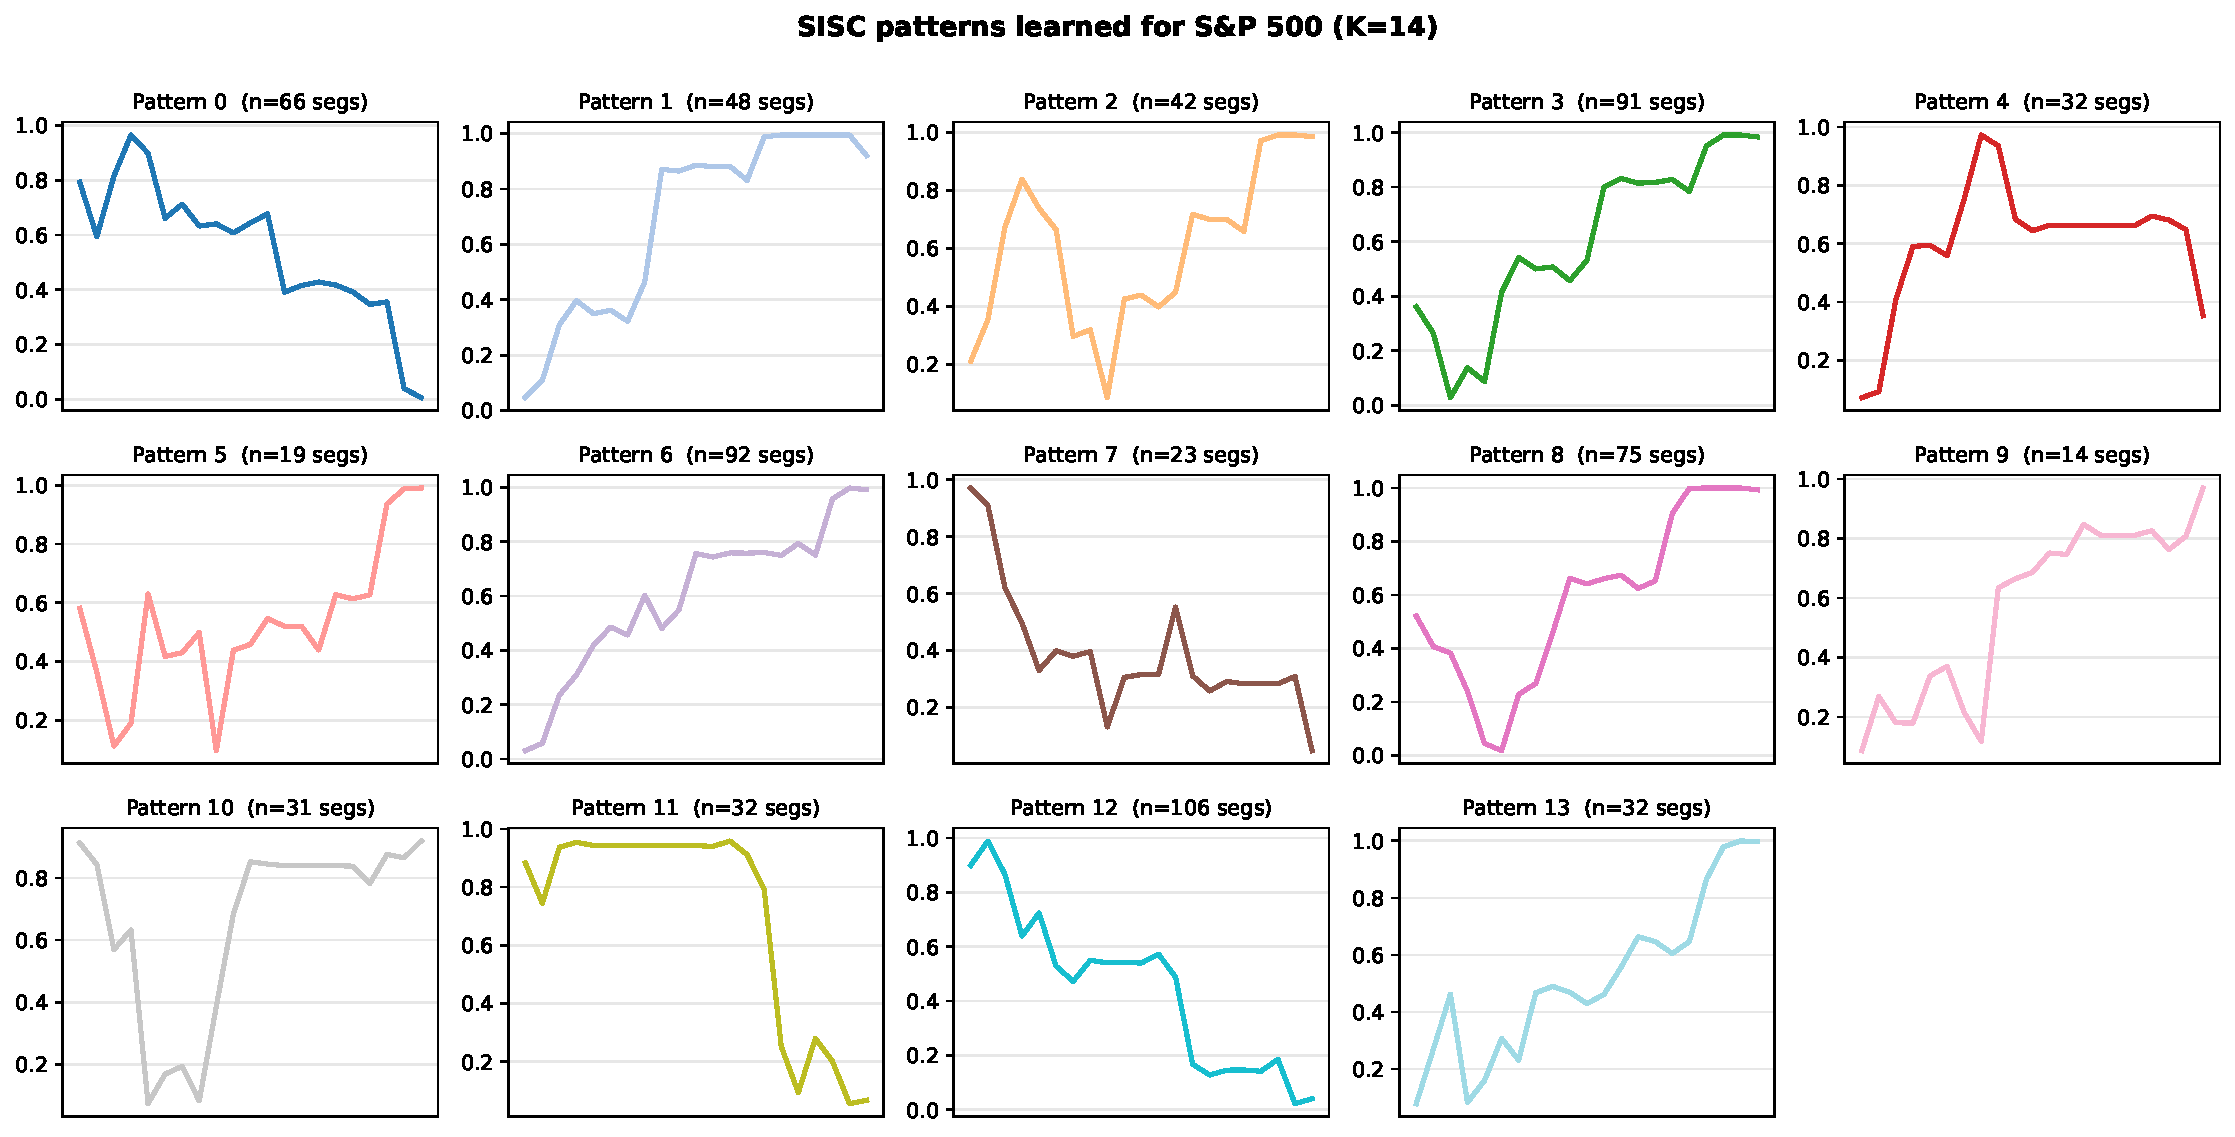
\includegraphics[width=0.88\textwidth]{figures/sisc/sp500/k14/patterns.pdf}
\note{S\&P 500 motifs learned by SISC with K=14. Visually: rebound, plateau, accelerated drawdown, and a clear head-and-shoulders shape around motifs 7--9. The K=14 setting is the one used in the paper. Centroid lengths span $[\lmin,\lmax]=[10,21]$ trading days.}
\end{frame}

\begin{frame}{S\&P 500 --- motif length / amplitude distribution}
\centering
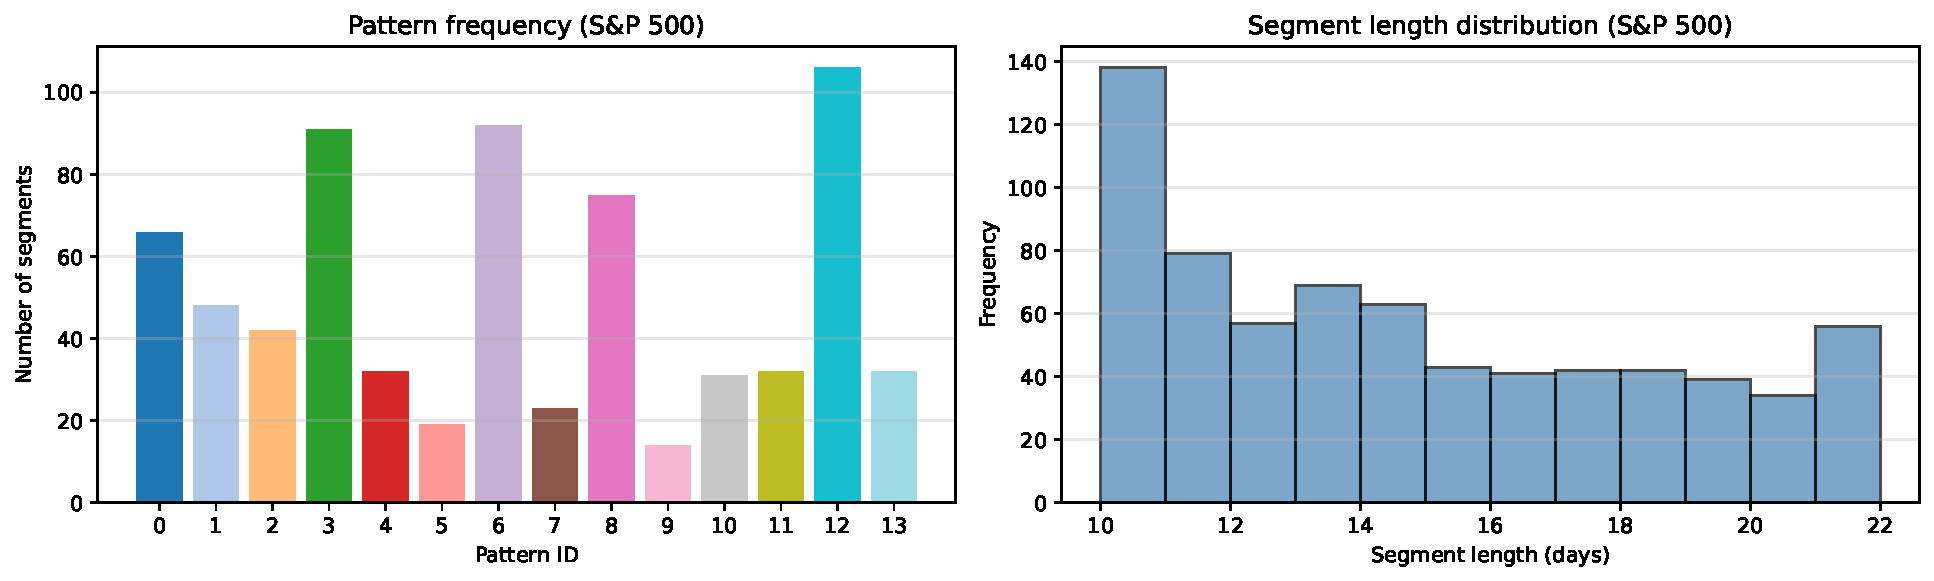
\includegraphics[width=0.88\textwidth]{figures/sisc/sp500/k14/pattern_stats.pdf}
\note{Per-motif statistics: how often each pattern occurs, its average duration, and its amplitude scale. A few motifs dominate occupancy --- the empirical motif distribution is far from uniform, which the evolution module needs to capture through the Markov chain.}
\end{frame}

\begin{frame}{GOOG --- learned motifs ($K=14$)}
\centering
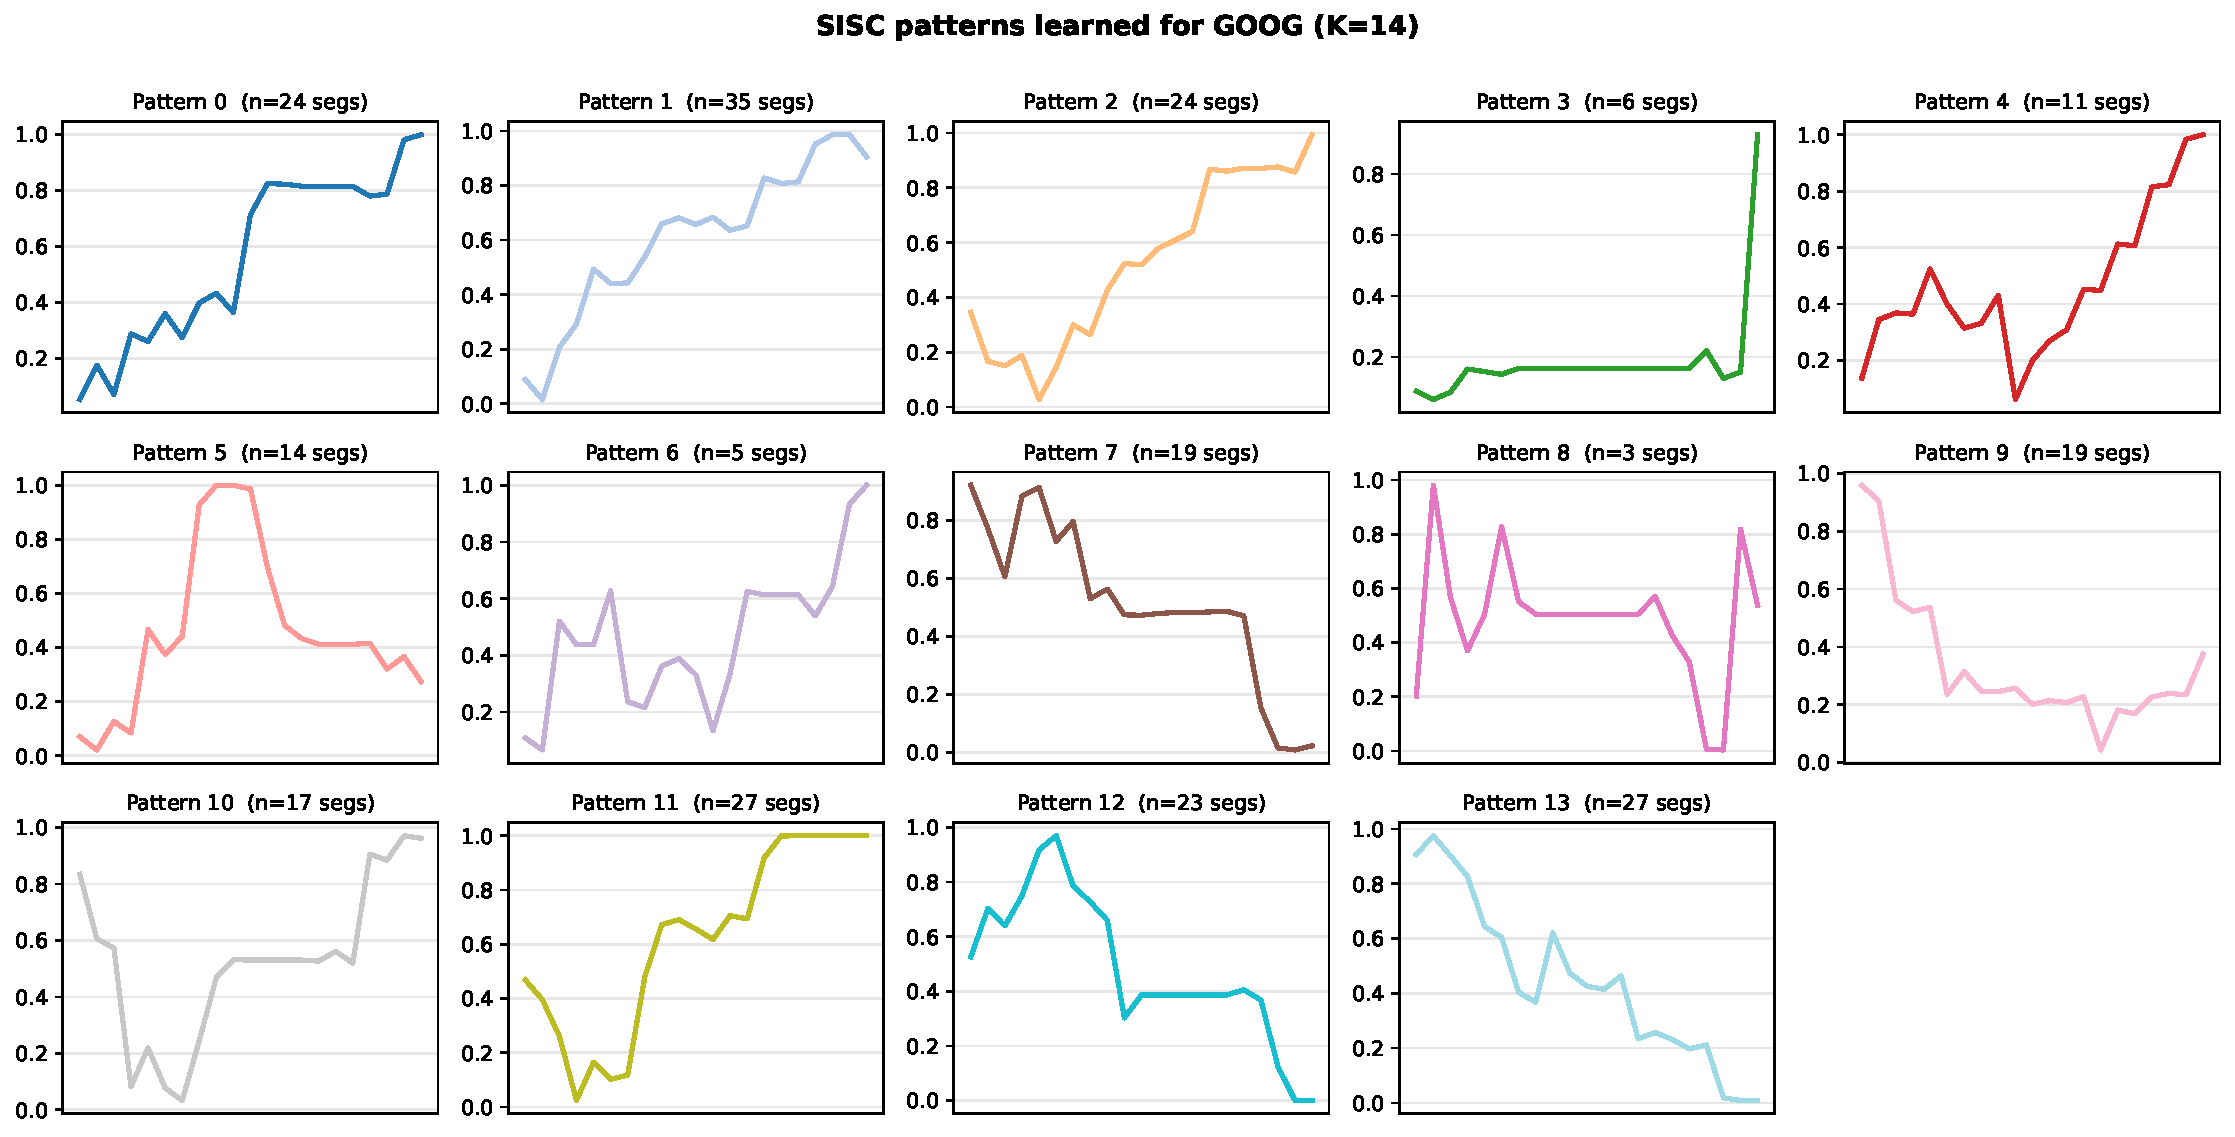
\includegraphics[width=0.88\textwidth]{figures/sisc/goog/k14/patterns.pdf}
\note{Google single-stock motifs at K=14. The motif library is qualitatively similar to S\&P 500 but with sharper amplitude swings consistent with single-name volatility. We see ascending and descending channels and a clear V-bottom near motifs 3 and 11.}
\end{frame}

\begin{frame}{GOOG --- learned motifs ($K=11$)}
\centering
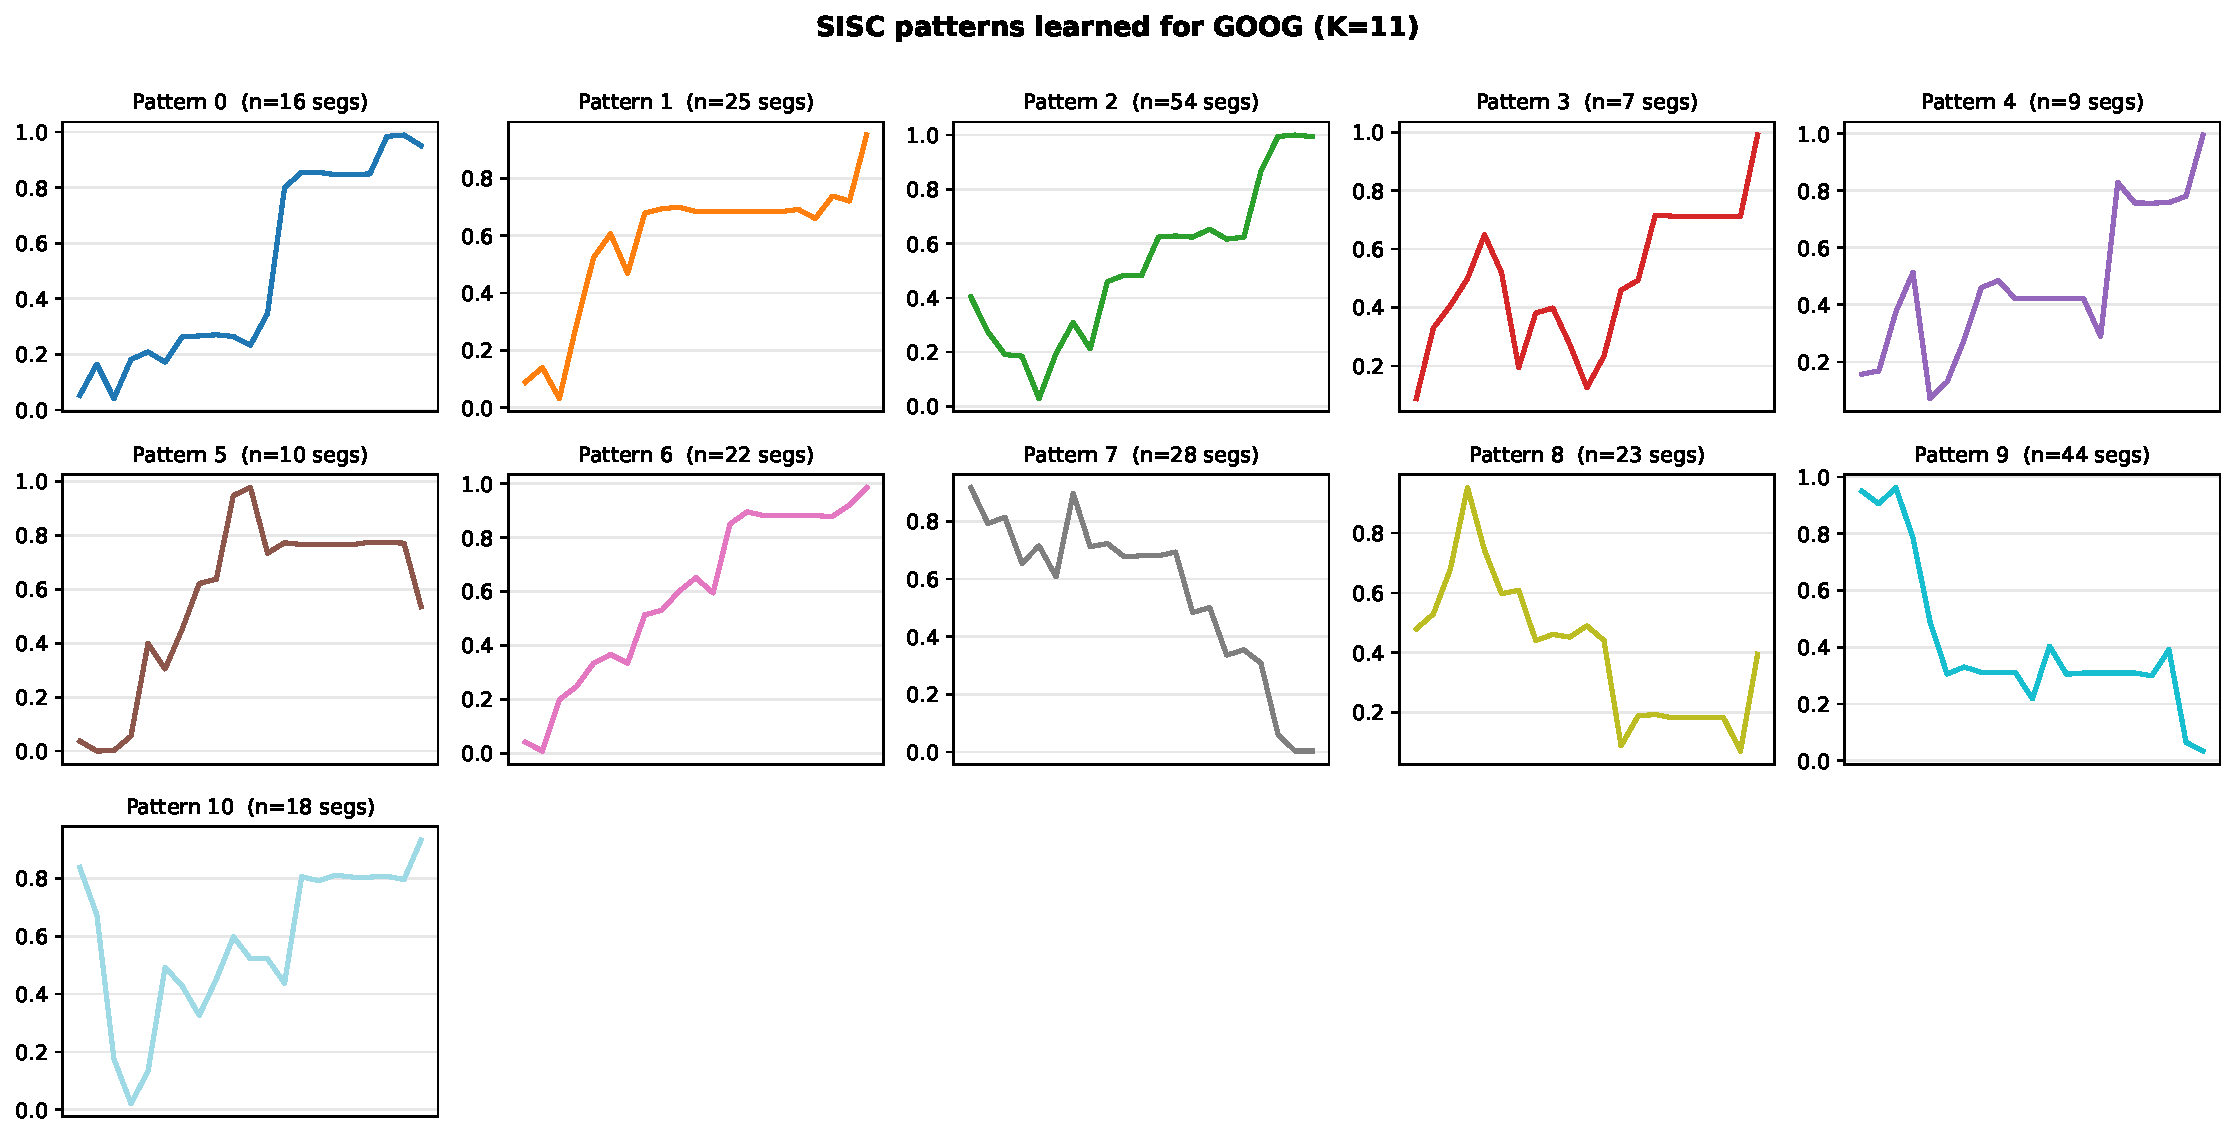
\includegraphics[width=0.88\textwidth]{figures/sisc/goog/k11/patterns.pdf}
\note{Same asset at K=11 for comparison. Reducing K from 14 to 11 collapses the head-and-shoulders subtypes into a single broader motif, illustrating how K trades resolution for cluster occupancy.}
\end{frame}

\begin{frame}{ZC=F --- learned motifs ($K=14$)}
\centering
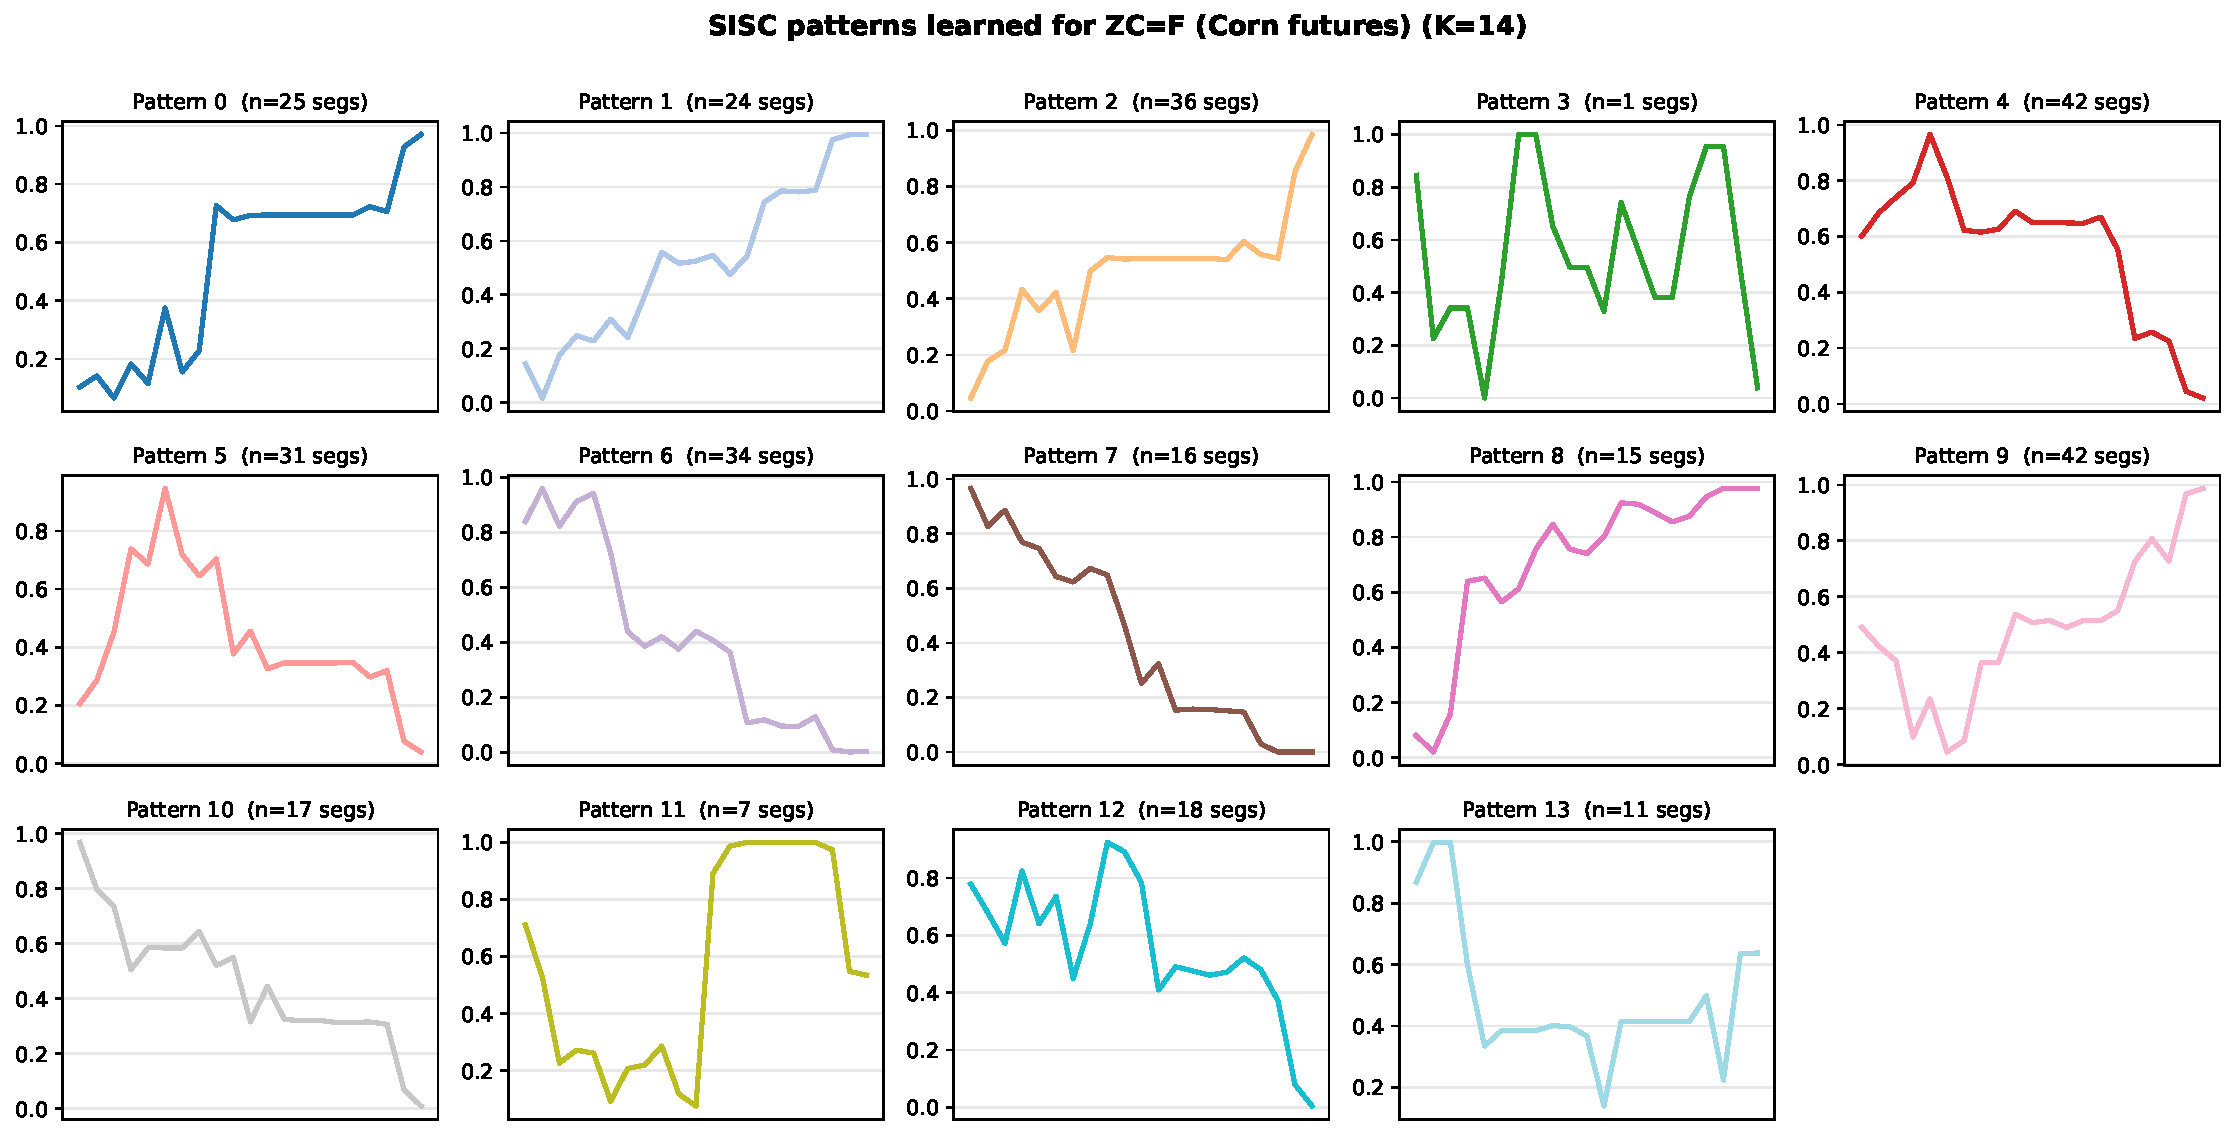
\includegraphics[width=0.88\textwidth]{figures/sisc/zcf/k14/patterns.pdf}
\note{Zero-coupon futures: a much shorter and noisier history than equity. The K=14 motif set is dominated by mean-reversion shapes; persistent trends are rarer, consistent with the underlying interest-rate dynamics.}
\end{frame}

\begin{frame}{ZC=F --- learned motifs ($K=13$)}
\centering
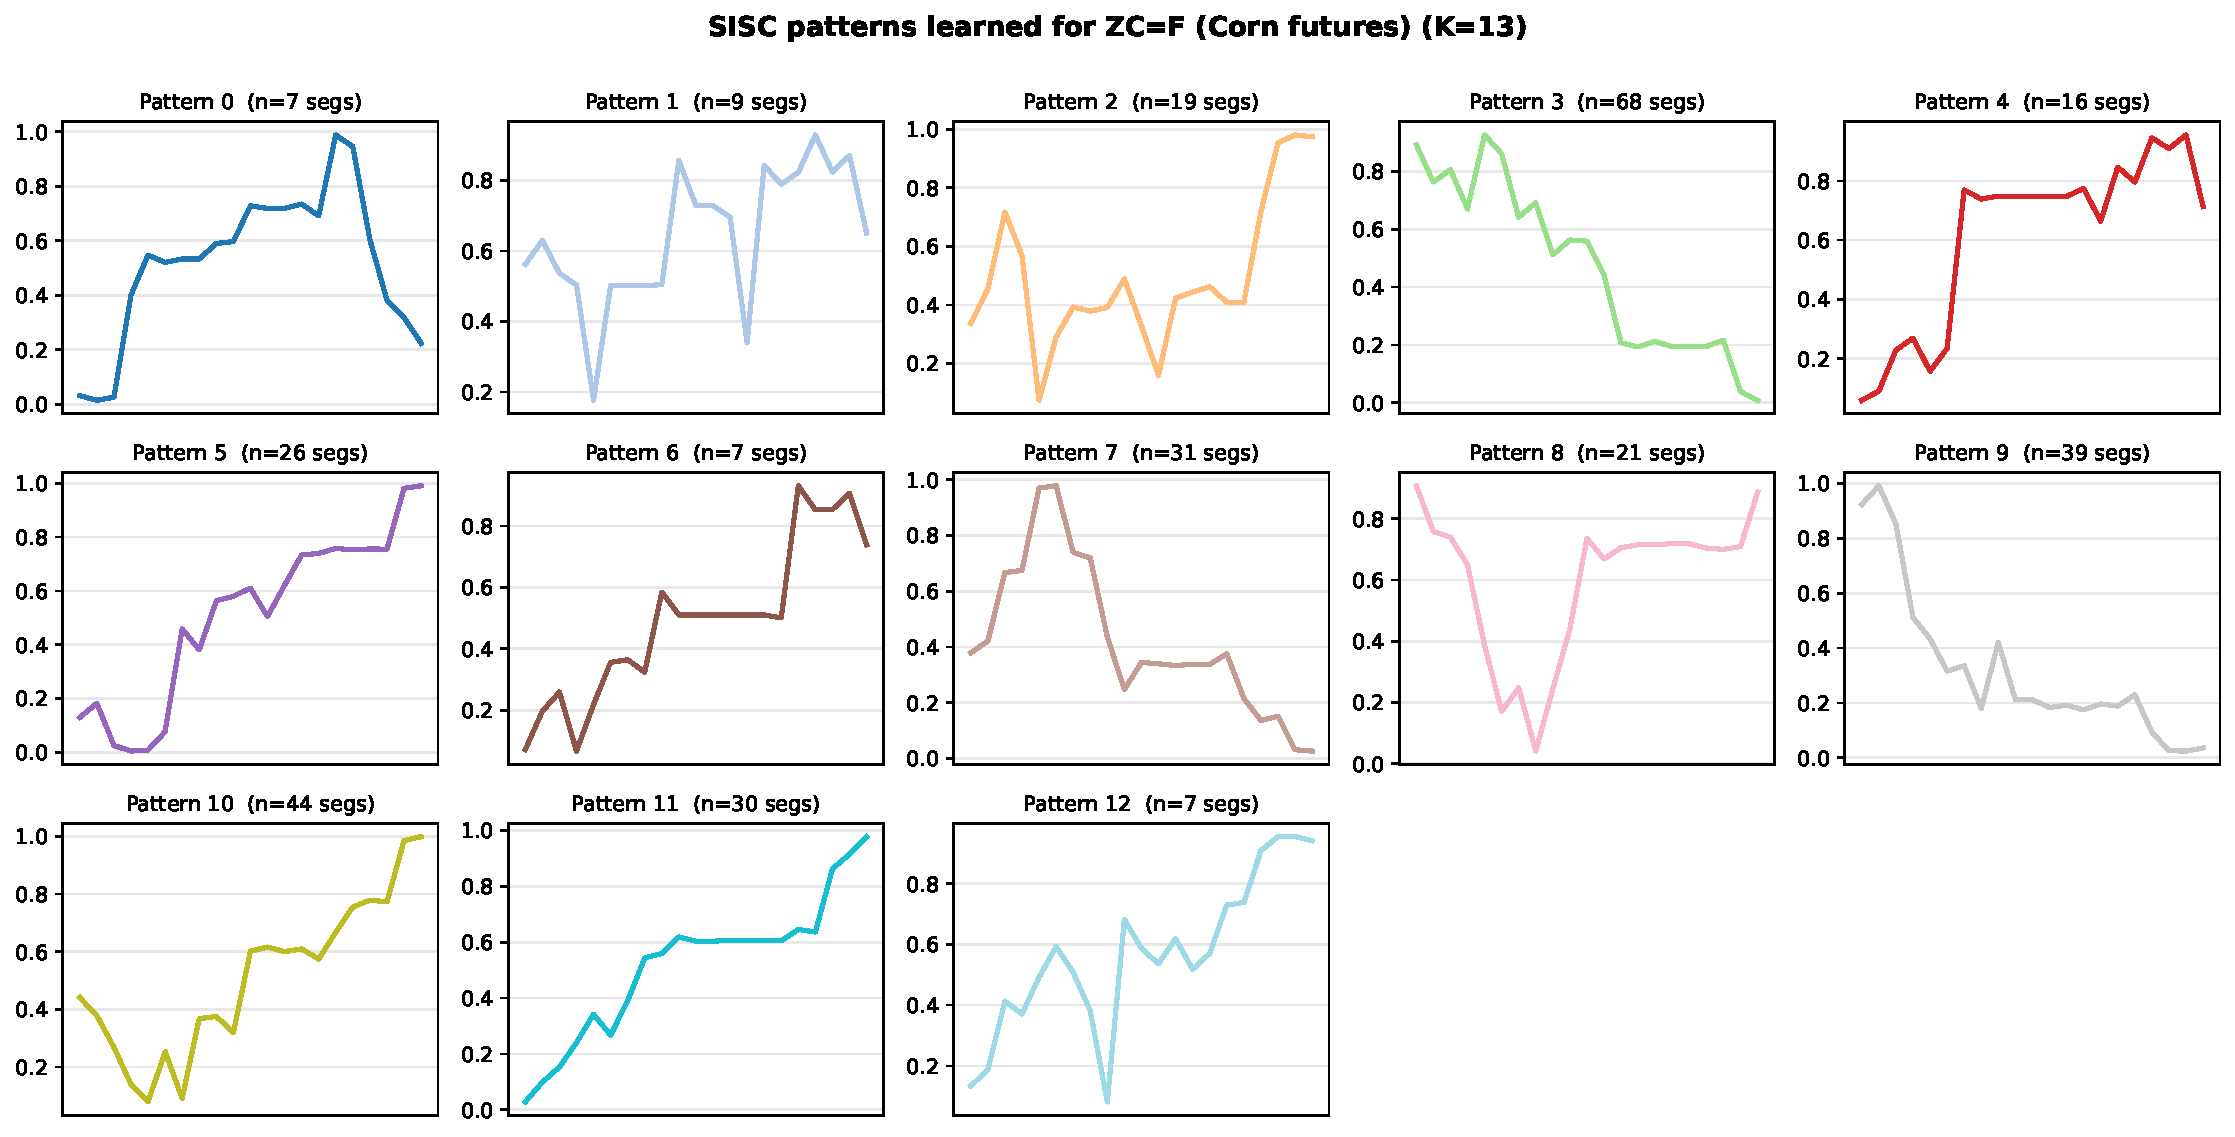
\includegraphics[width=0.88\textwidth]{figures/sisc/zcf/k13/patterns.pdf}
\note{K=13 was reported by the authors for ZC=F. The visual library matches K=14 closely --- the marginal motif at K=14 is a near-duplicate of motif 9, suggesting K=13 is close to optimal under the elbow heuristic.}
\end{frame}

\begin{frame}{ZC=F --- learned motifs ($K=11$)}
\centering
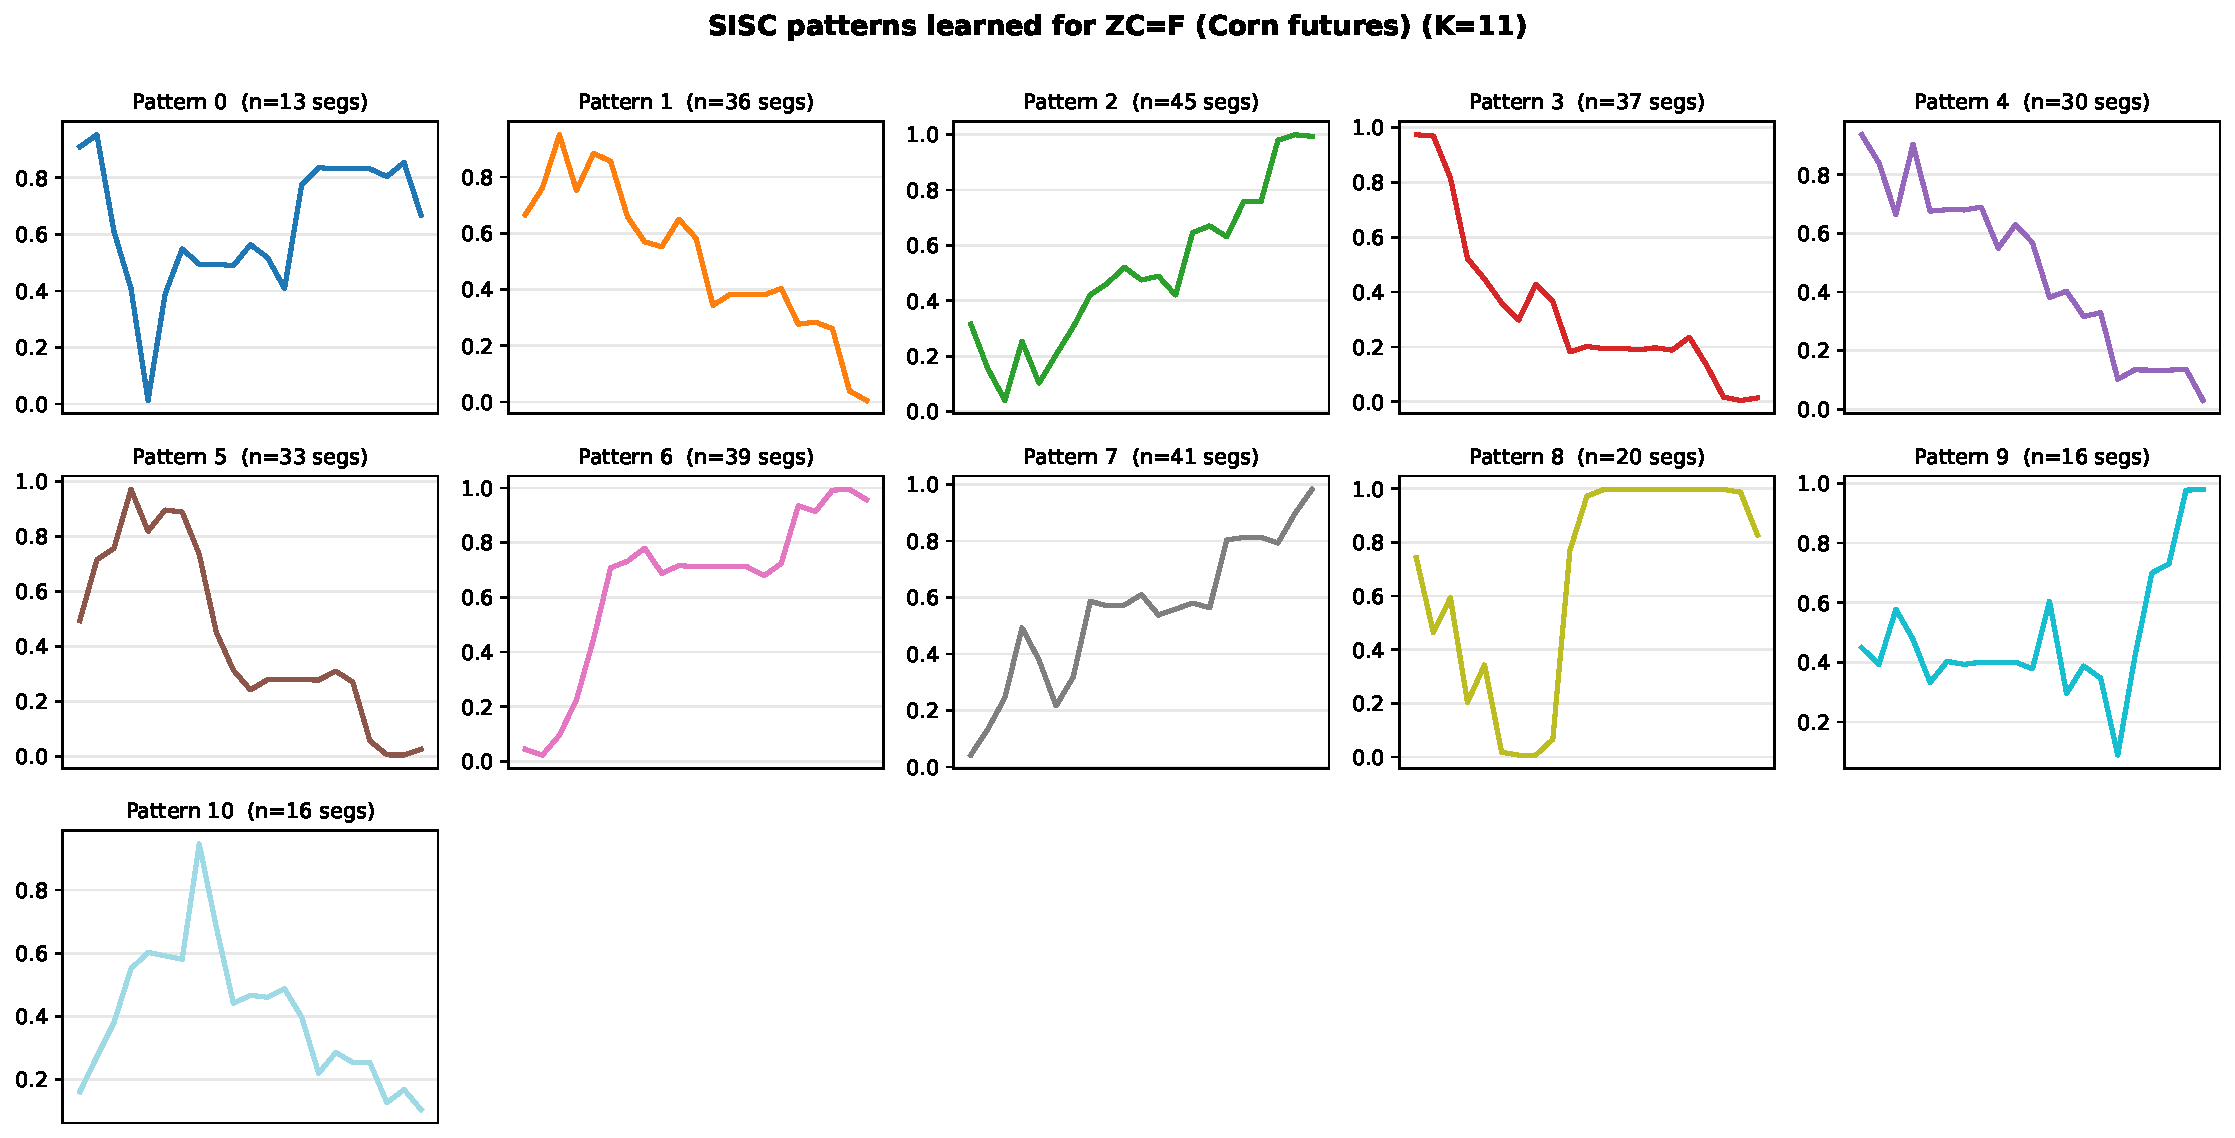
\includegraphics[width=0.88\textwidth]{figures/sisc/zcf/k11/patterns.pdf}
\note{K=11 collapses two of the smaller mean-reversion shapes into a single broader motif. Useful as a sensitivity check: downstream MAPE will allow us to compare K=11/13/14 quantitatively.}
\end{frame}

% =====================================================================
\section{Downstream TATR experiments}
% =====================================================================

\begin{frame}{TATR --- S\&P 500, paper-faithful style}
\centering
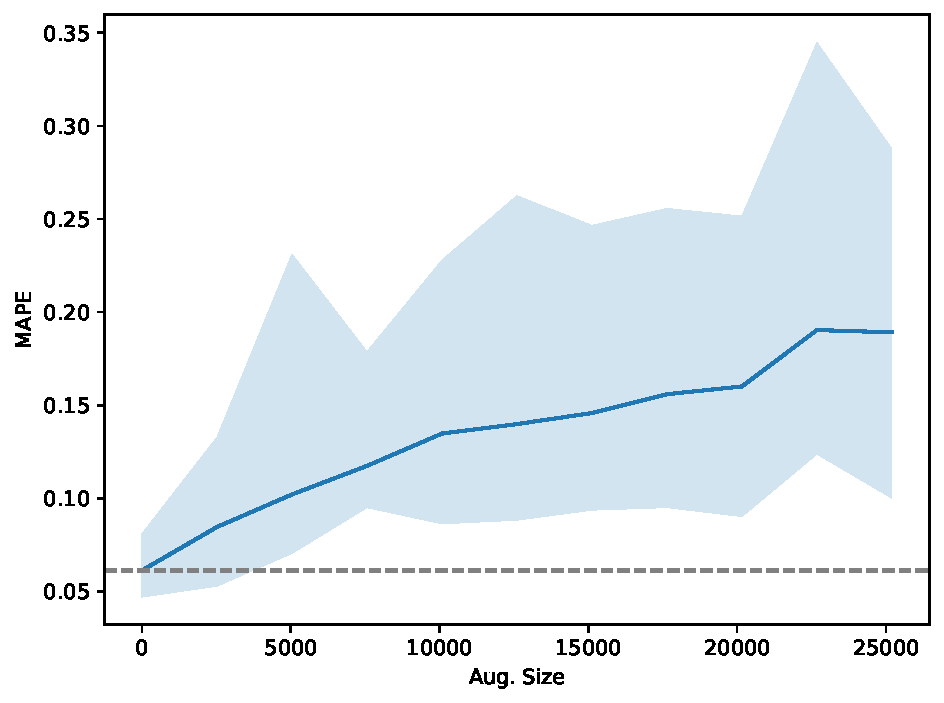
\includegraphics[width=0.78\textwidth]{figures/tatr/sp500/k14/authors/final.pdf}
\note{TATR replicates the augmentation experiment from the paper: training a small LSTM on real-plus-synthetic data and comparing MAPE against real-only baseline. Authors' protocol on S\&P 500. The qualitative shape of the curve matches Figure~6b of the paper, but the absolute MAPE is consistently higher, which is the first hint that something protocol-related is off.}
\end{frame}

\begin{frame}{TATR --- S\&P 500, diagnostic (with CIs and \% vs paper)}
\centering
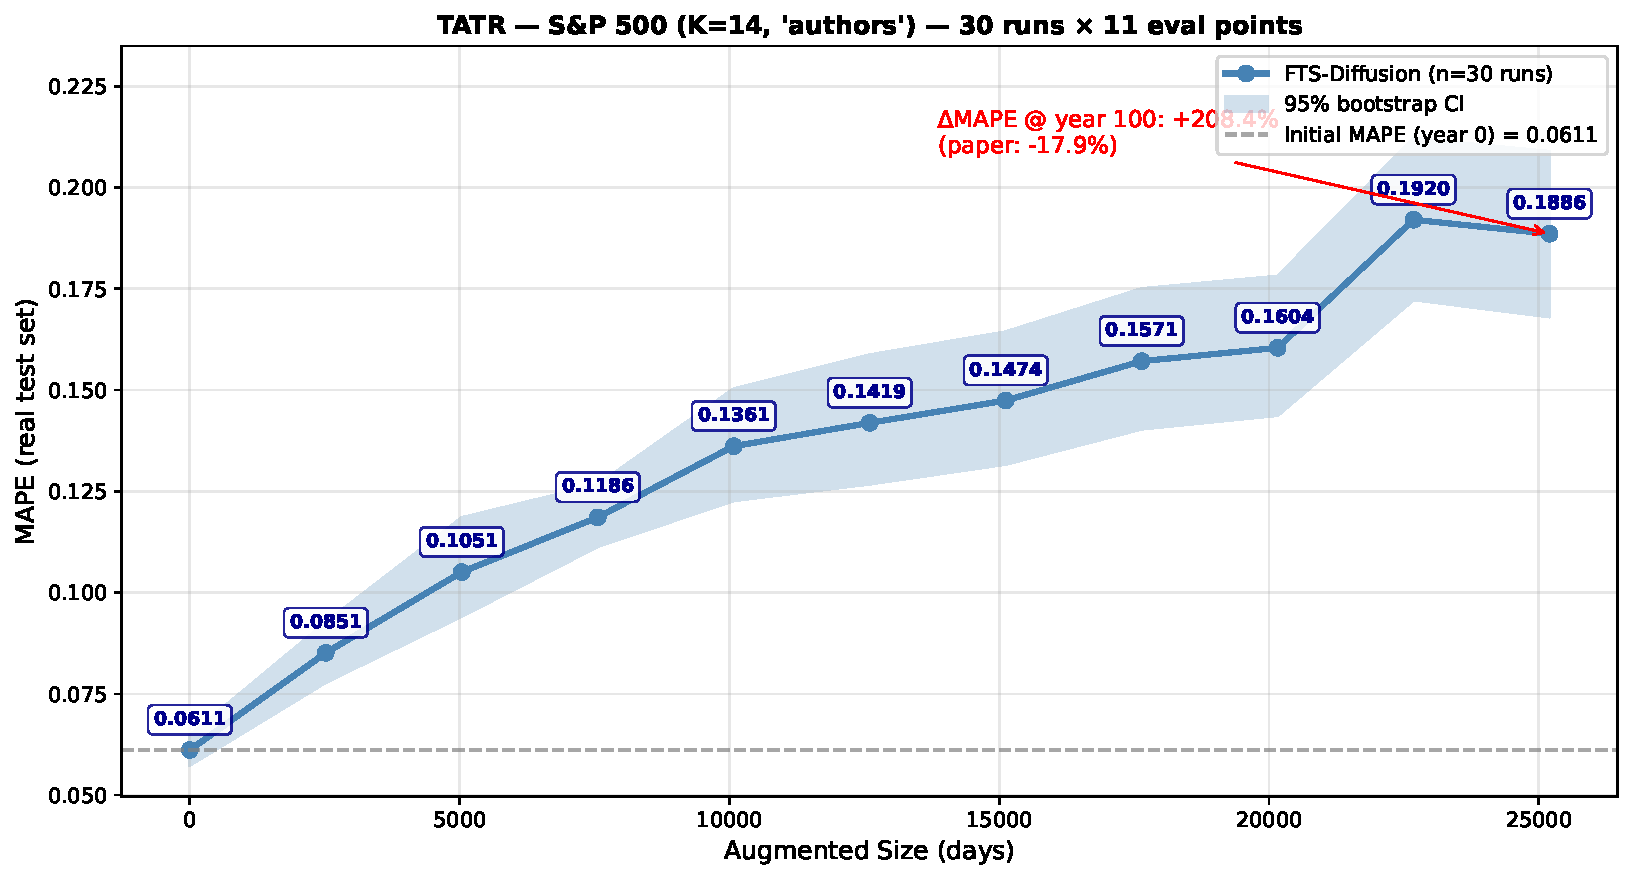
\includegraphics[width=0.78\textwidth]{figures/tatr/sp500/k14/authors/final_enhanced.pdf}
\note{Our enhanced version adds 90\% bootstrap confidence intervals over 30 runs and the percentage gap versus the published Figure~6b numbers. Two observations: (i)~variance is much larger than the paper suggests; (ii)~MAPE \alert{grows} with augmentation under the authors' protocol on S\&P 500 --- the opposite of the published trend.}
\end{frame}

\begin{frame}{TATR --- S\&P 500, single vs random\_init protocols}
\centering
\begin{columns}[T,onlytextwidth]
  \column{0.50\textwidth}
    \centering\footnotesize \textbf{Single}\\[1mm]
    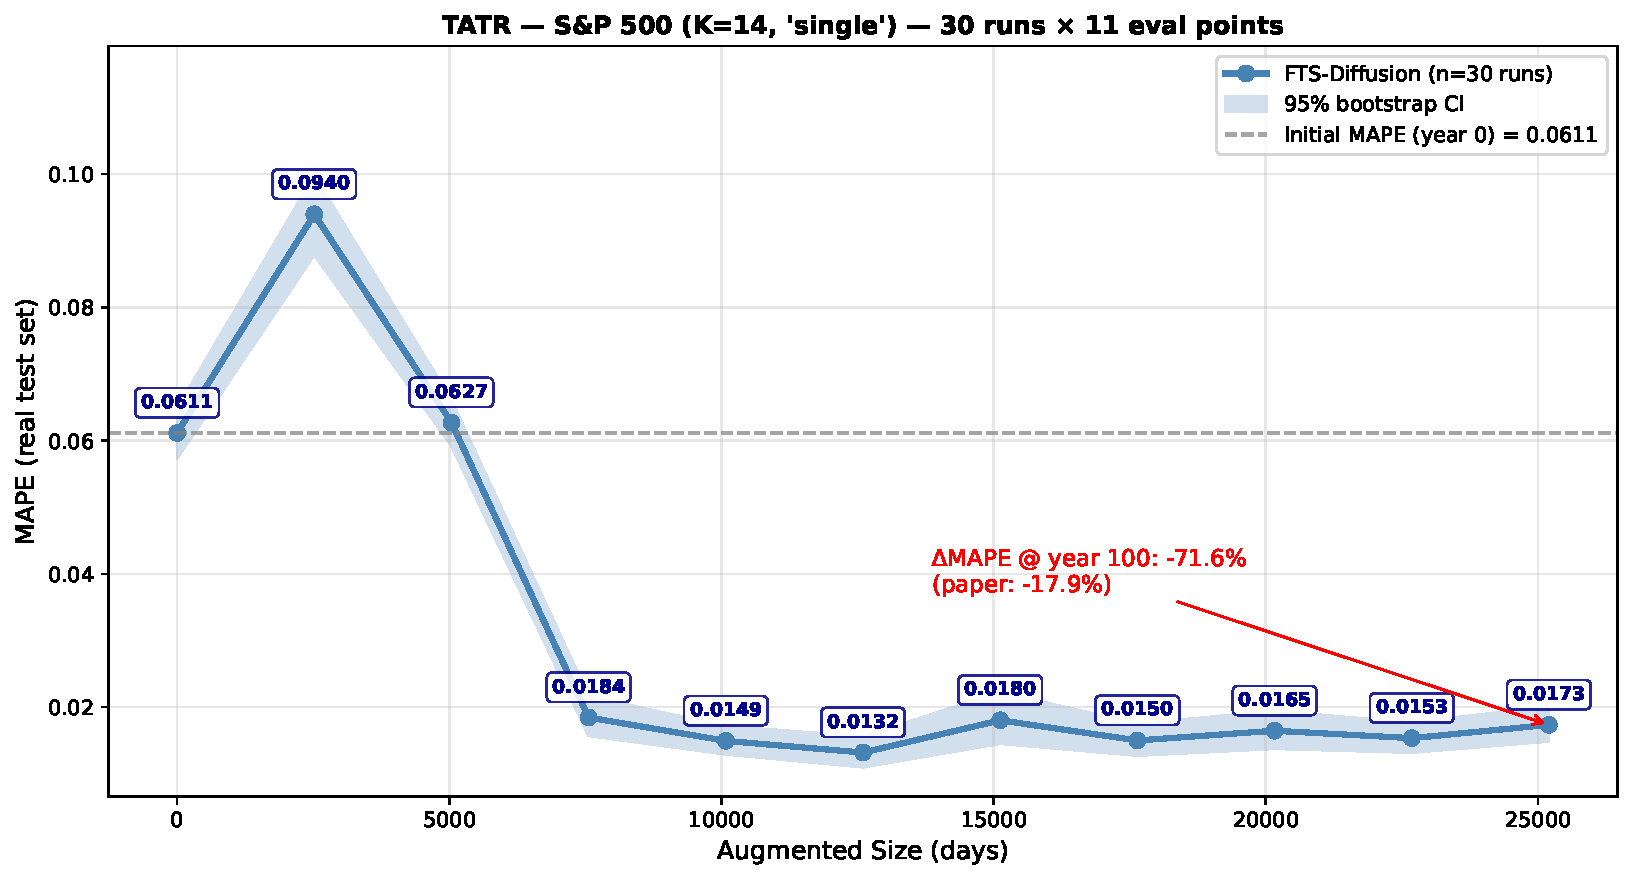
\includegraphics[width=\linewidth]{figures/tatr/sp500/k14/single/final_enhanced.pdf}
  \column{0.50\textwidth}
    \centering\footnotesize \textbf{Random init}\\[1mm]
    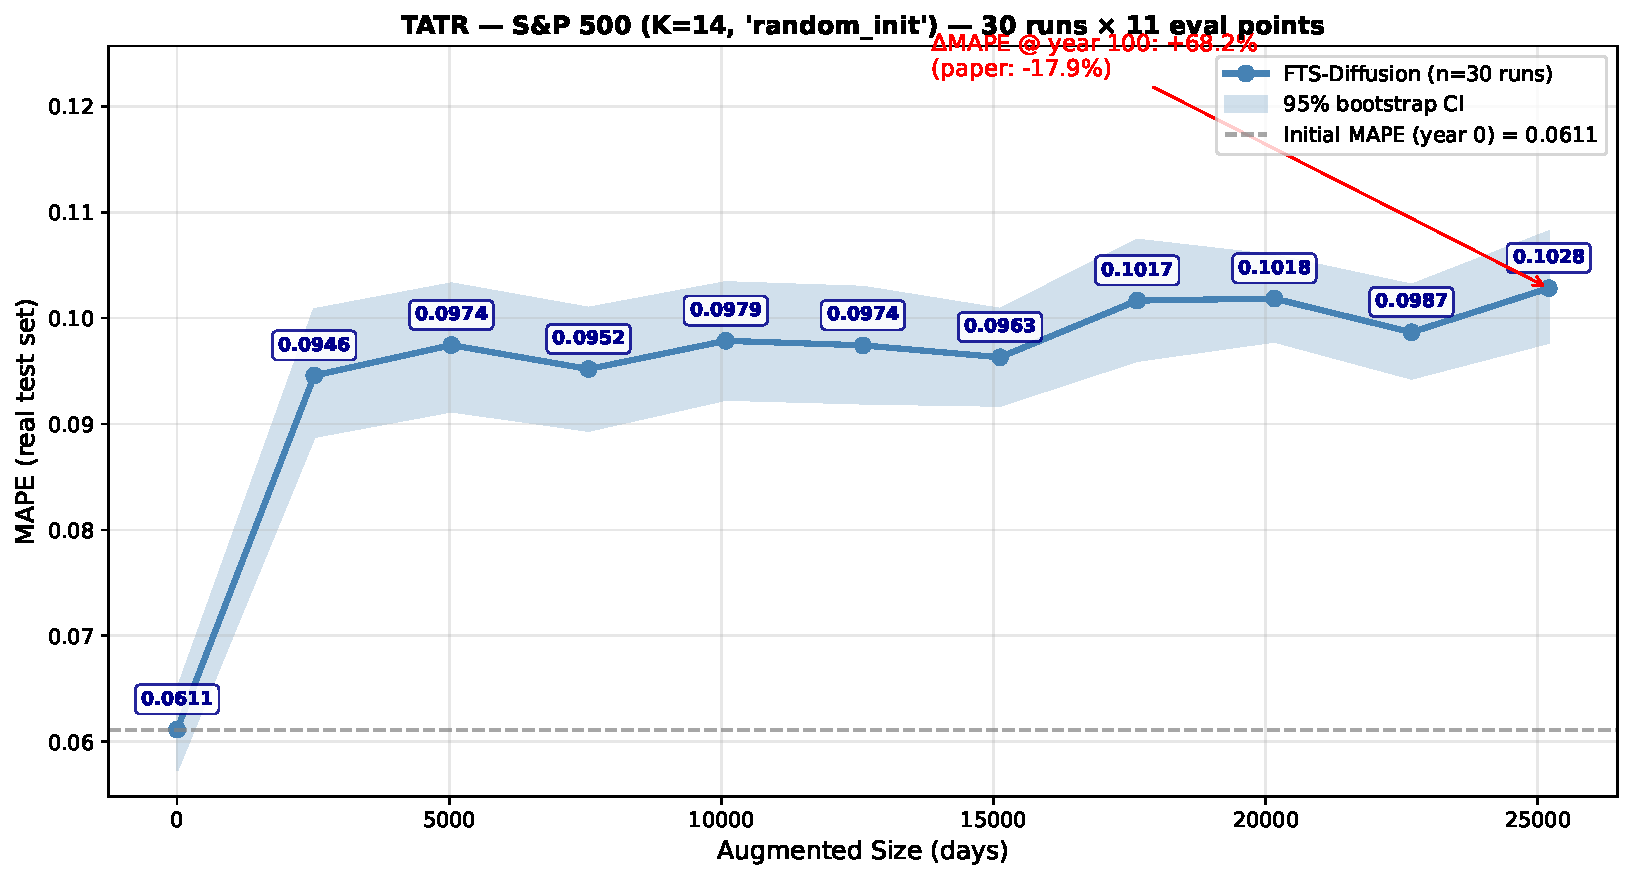
\includegraphics[width=\linewidth]{figures/tatr/sp500/k14/random_init/final_enhanced.pdf}
\end{columns}
\note{Two alternative protocols on S\&P 500. The \texttt{single} protocol re-uses one long synthetic series; \texttt{random\_init} starts each rolling window from a fresh historical initial segment. Random\_init is the closest match to the published curve --- a hint that the paper's protocol is closer to random\_init than to authors' description.}
\end{frame}

\begin{frame}{TATR --- GOOG, paper-faithful style}
\centering
\begin{columns}[T,onlytextwidth]
  \column{0.50\textwidth}
    \centering\footnotesize \textbf{$K=14$, authors}\\[1mm]
    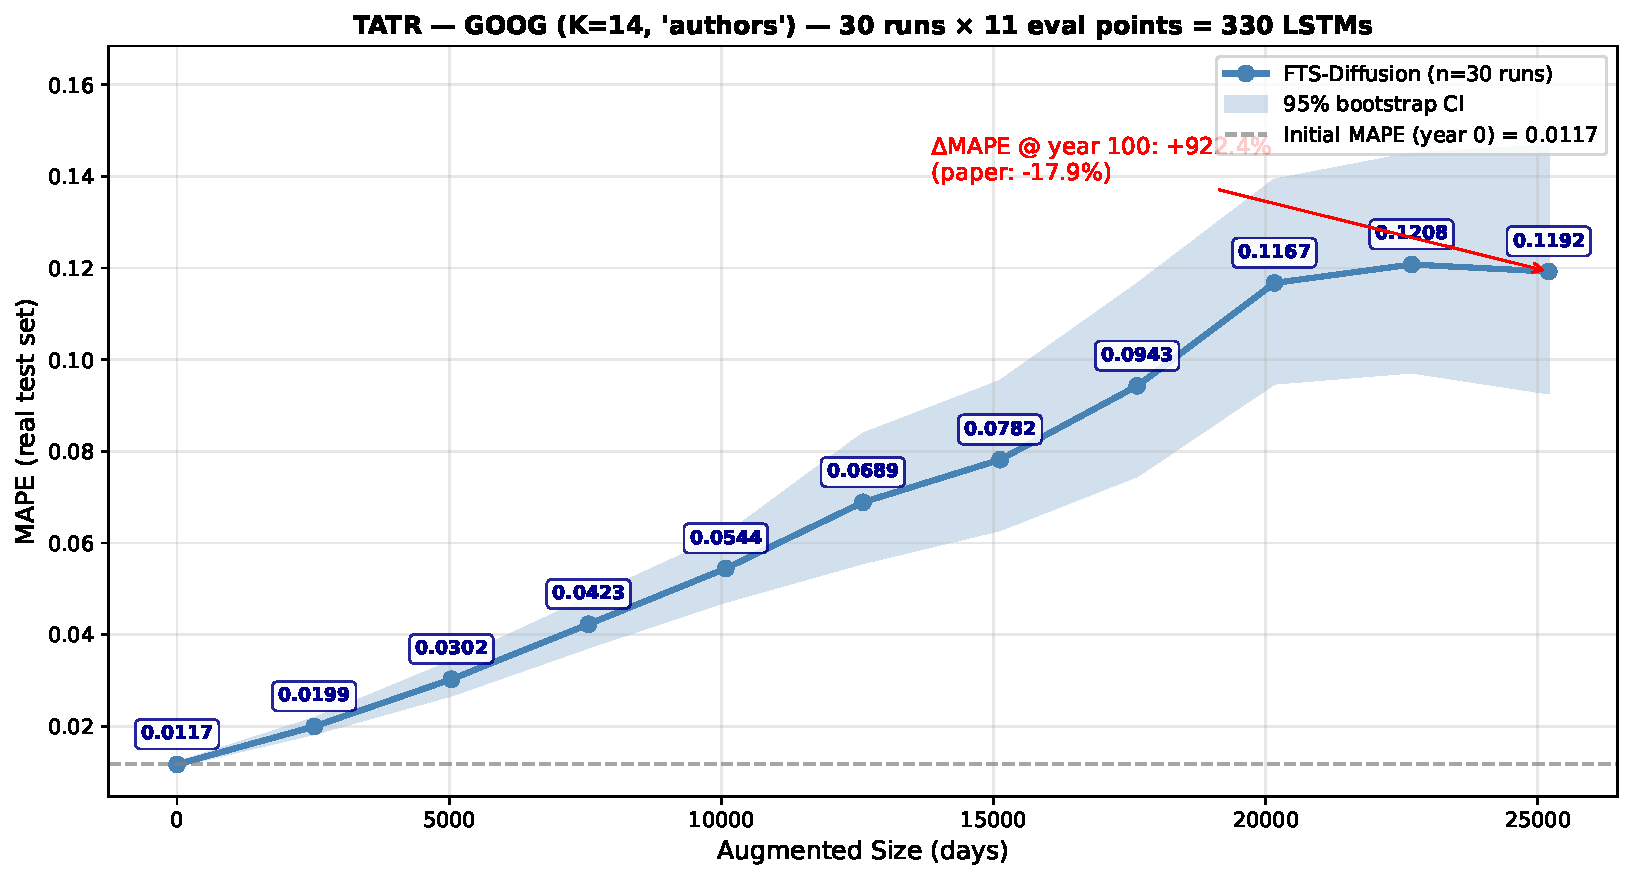
\includegraphics[width=\linewidth]{figures/tatr/goog/k14/authors/final.pdf}
  \column{0.50\textwidth}
    \centering\footnotesize \textbf{$K=11$, authors}\\[1mm]
    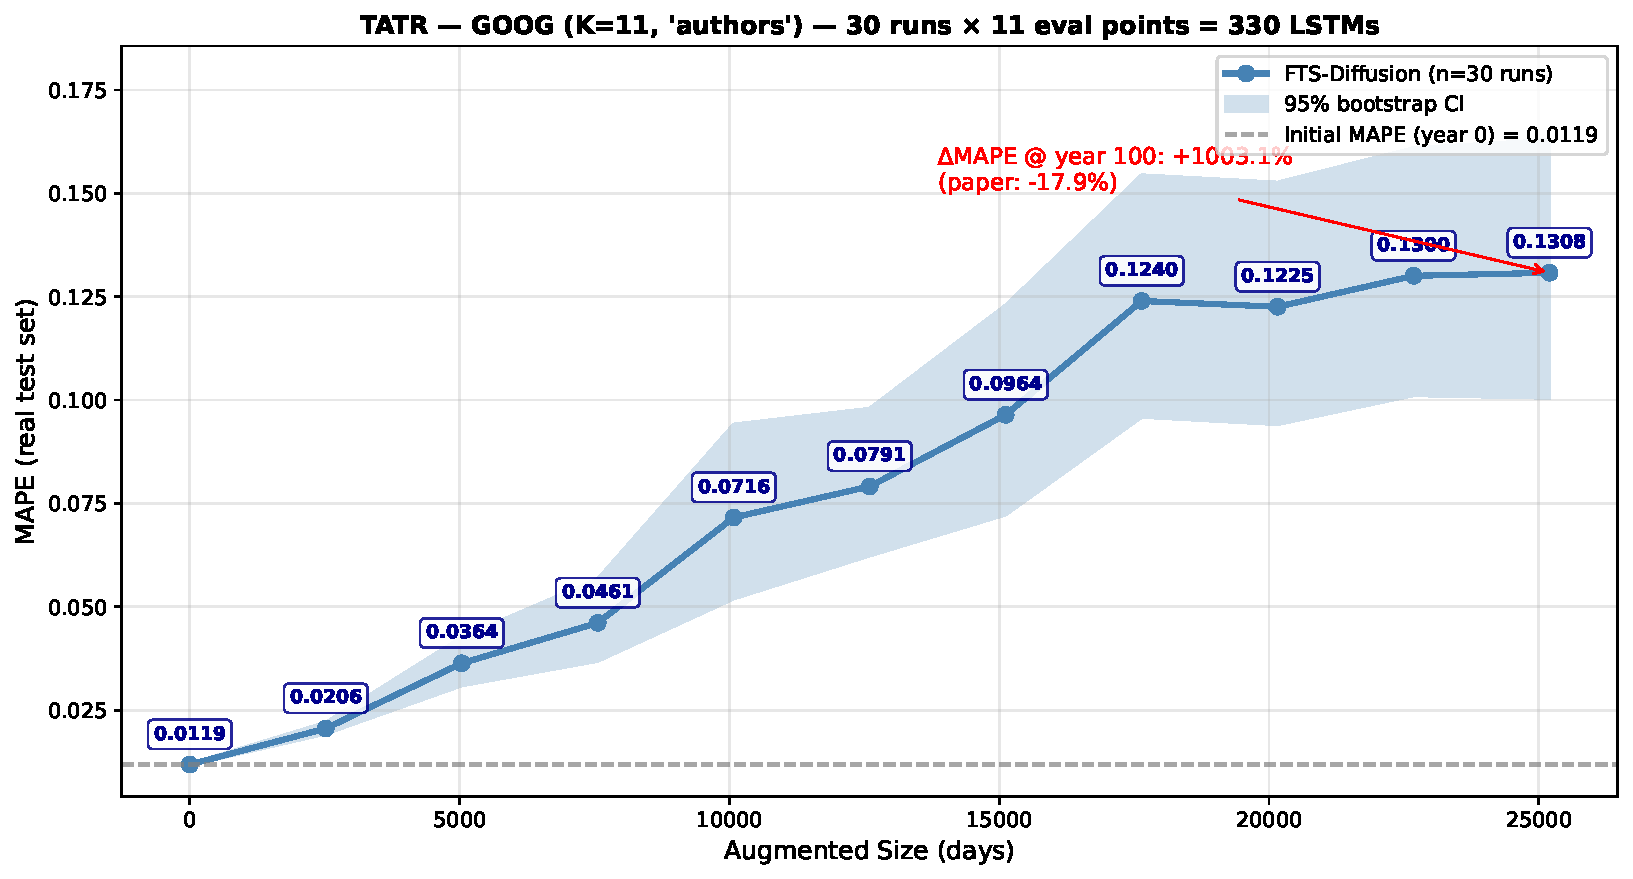
\includegraphics[width=\linewidth]{figures/tatr/goog/k11/authors/final.pdf}
\end{columns}
\note{GOOG, authors' protocol, at the two cluster counts. Both curves drift upward with augmentation: the synthetic data degrades, not helps, the downstream LSTM. K does not change the qualitative picture.}
\end{frame}

\begin{frame}{TATR --- GOOG, diagnostic enhanced}
\centering
\begin{columns}[T,onlytextwidth]
  \column{0.50\textwidth}
    \centering\footnotesize \textbf{$K=14$, single}\\[1mm]
    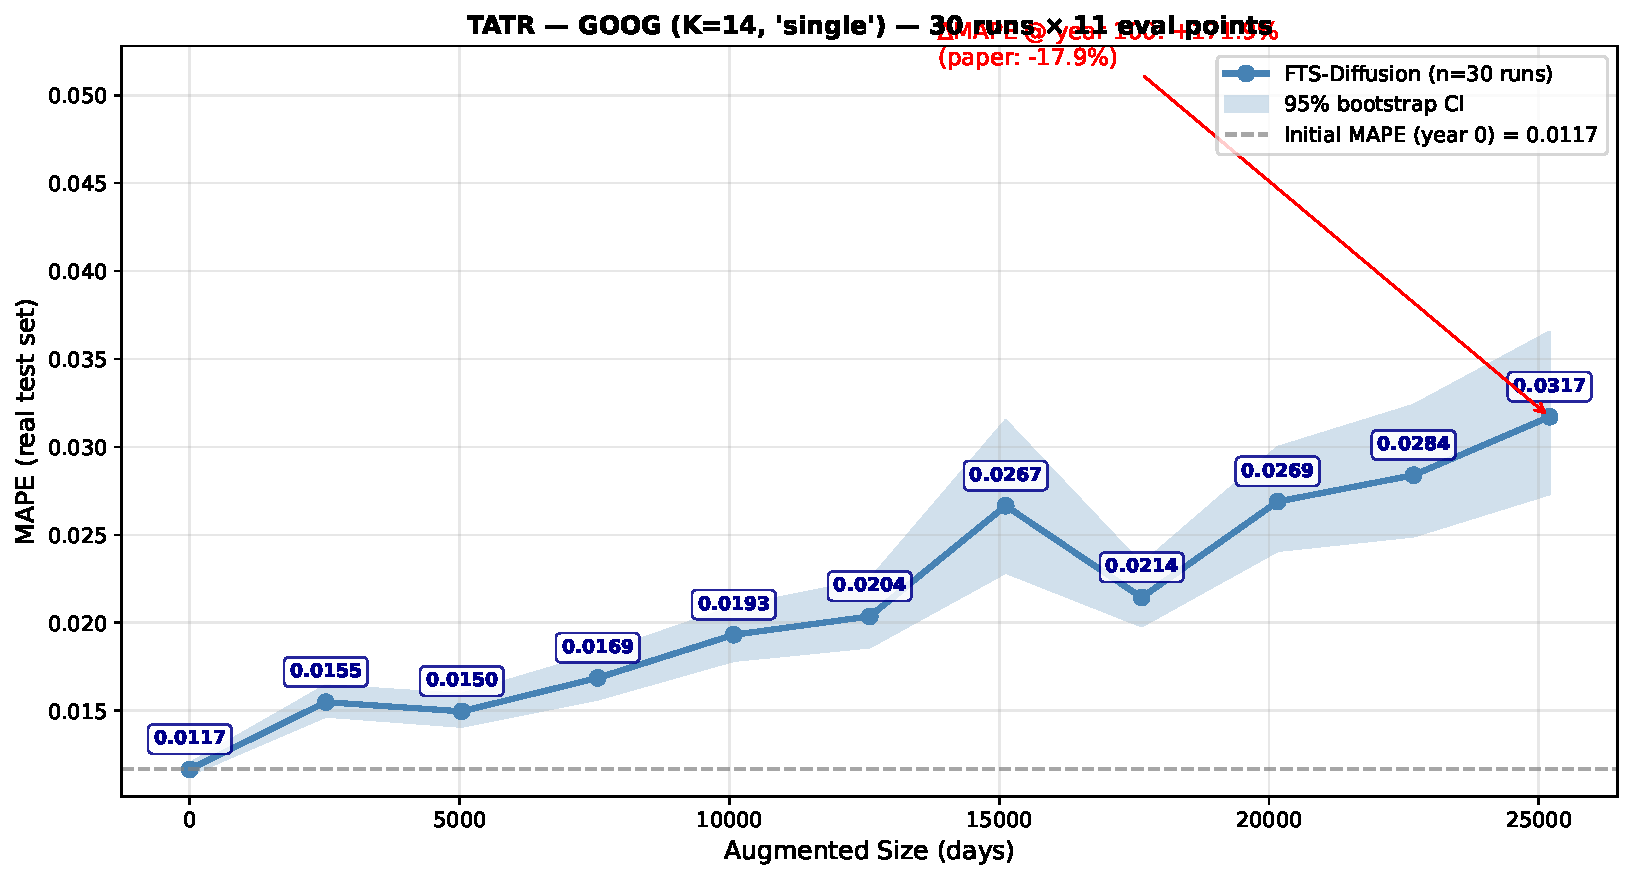
\includegraphics[width=\linewidth]{figures/tatr/goog/k14/single/final_enhanced.pdf}
  \column{0.50\textwidth}
    \centering\footnotesize \textbf{$K=11$, single}\\[1mm]
    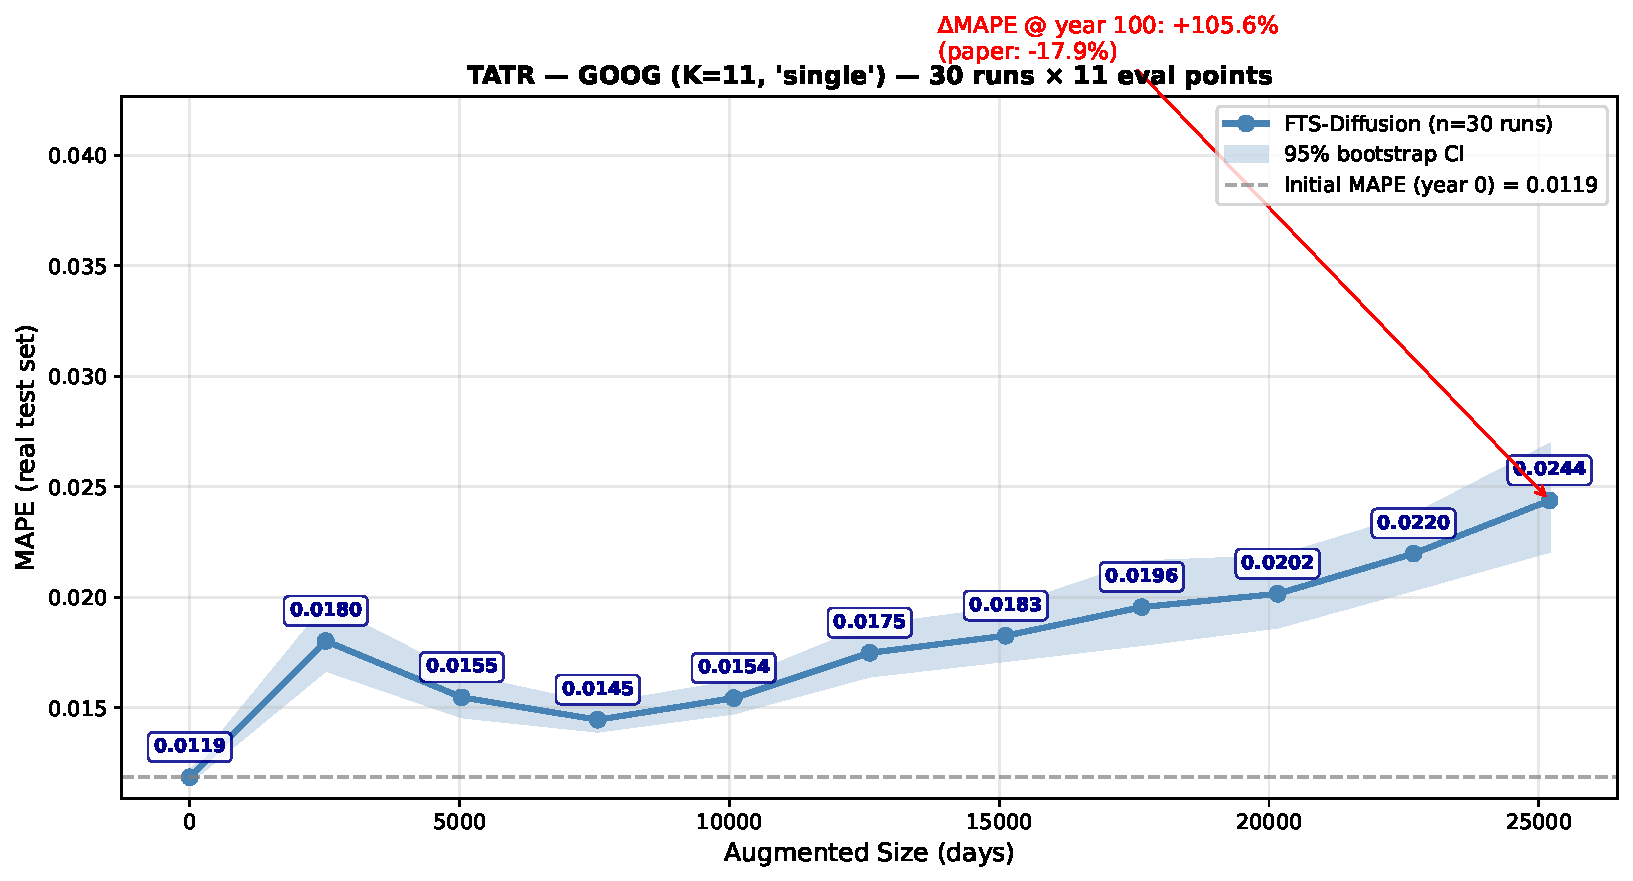
\includegraphics[width=\linewidth]{figures/tatr/goog/k11/single/final_enhanced.pdf}
\end{columns}
\note{Same asset with the \texttt{single} protocol and enhanced annotations. The variance bands tighten compared to authors' protocol, but the MAPE-grows-with-augmentation effect remains. Aspect-ratio of the bug: persistent across protocols.}
\end{frame}

\begin{frame}{TATR --- ZC=F, paper-faithful style}
\centering
\begin{columns}[T,onlytextwidth]
  \column{0.50\textwidth}
    \centering\footnotesize \textbf{$K=14$}\\[1mm]
    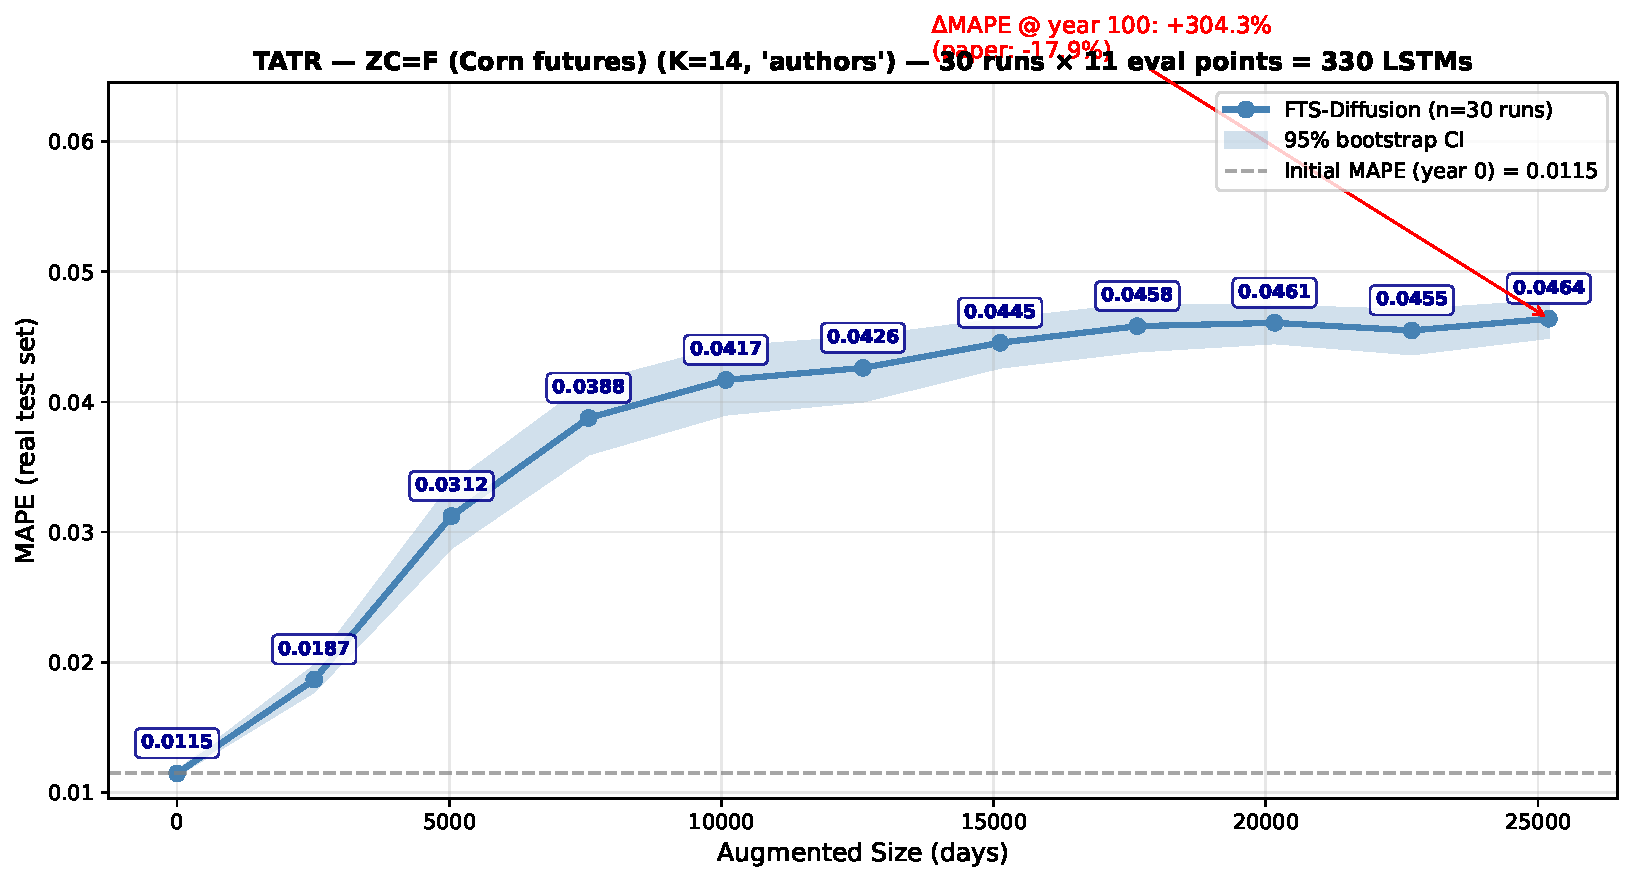
\includegraphics[width=\linewidth]{figures/tatr/zcf/k14/authors/final.pdf}
  \column{0.50\textwidth}
    \centering\footnotesize \textbf{$K=13$ (paper's $K$)}\\[1mm]
    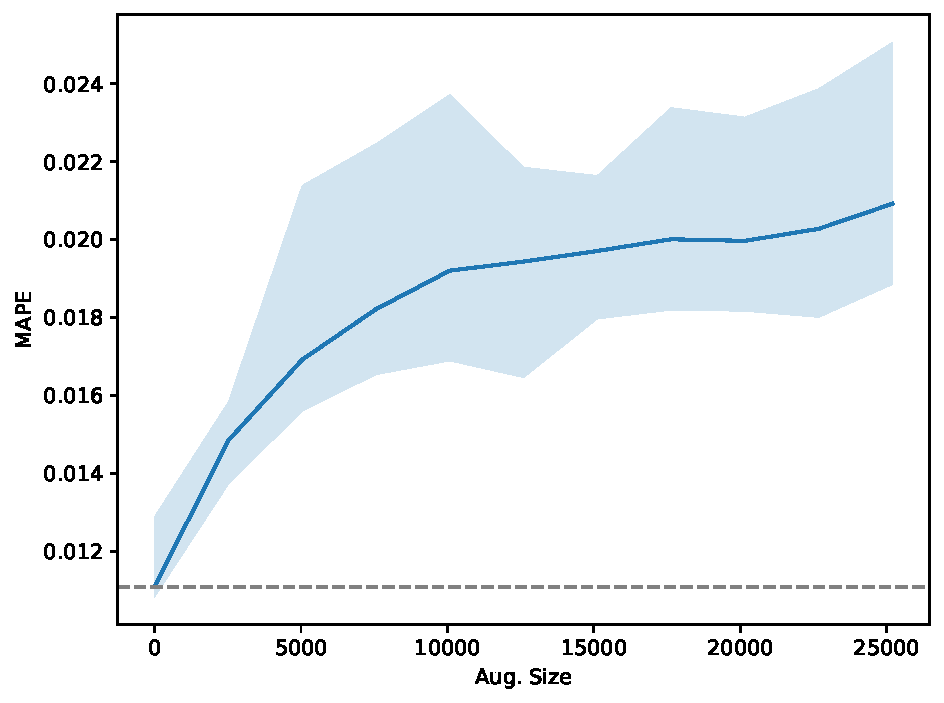
\includegraphics[width=\linewidth]{figures/tatr/zcf/k13/authors/final.pdf}
\end{columns}
\note{ZC=F is the asset where the published result is most striking. We reproduce the down-sloping MAPE curve at K=13 (paper's choice), but with a much smaller magnitude than reported. K=14 is similar; K=11 (next slide) is qualitatively different.}
\end{frame}

\begin{frame}{TATR --- ZC=F, diagnostic enhanced}
\centering
\begin{columns}[T,onlytextwidth]
  \column{0.50\textwidth}
    \centering\footnotesize \textbf{$K=14$, single}\\[1mm]
    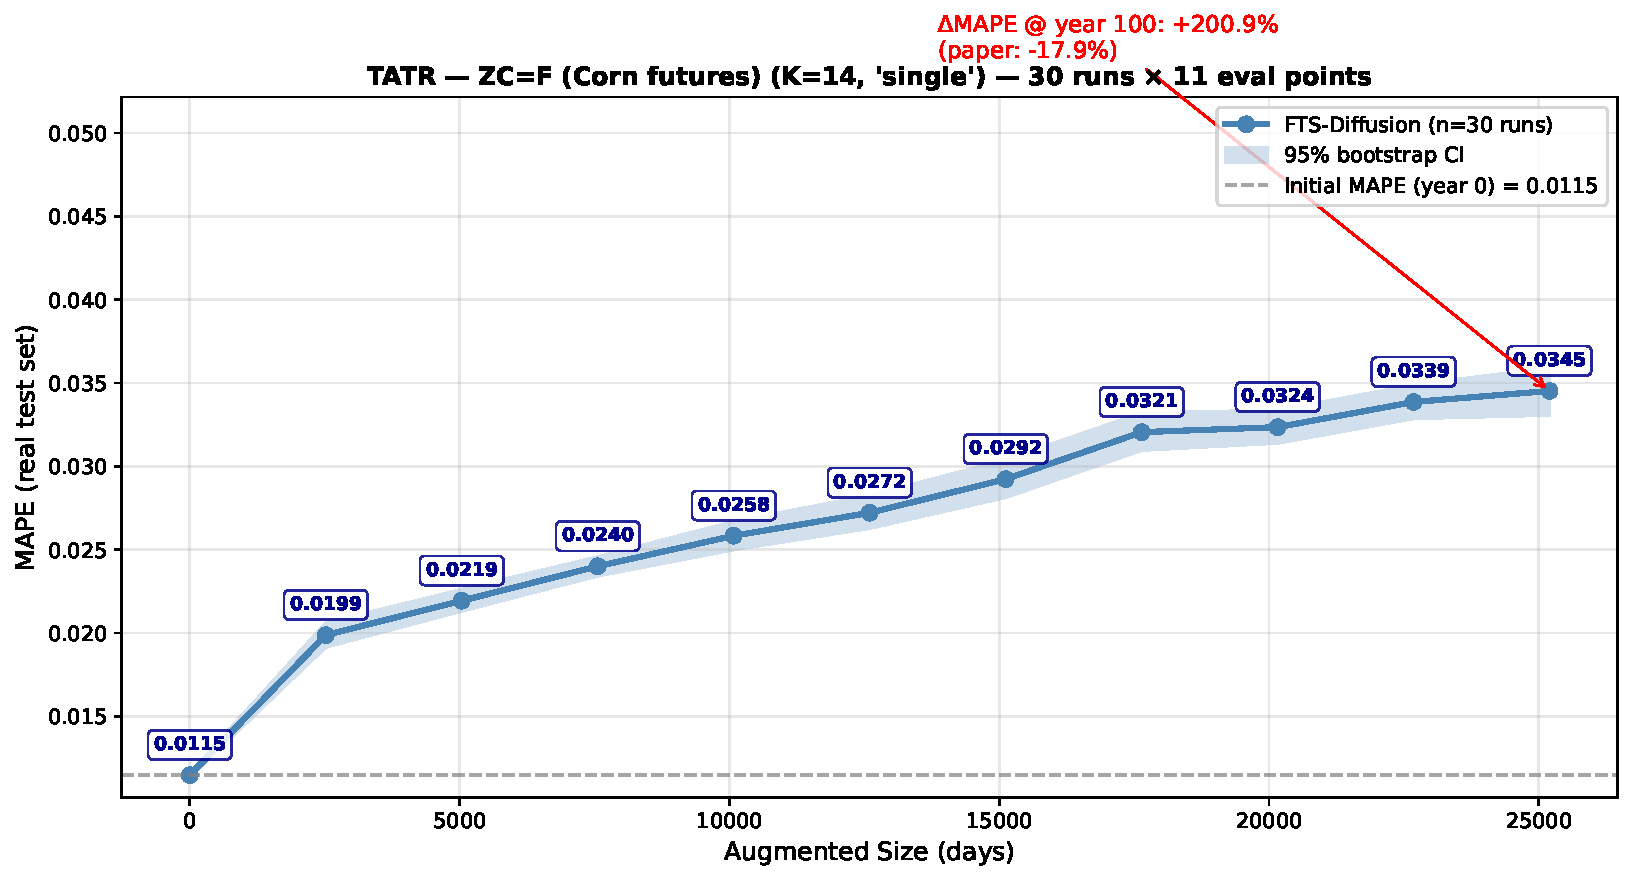
\includegraphics[width=\linewidth]{figures/tatr/zcf/k14/single/final_enhanced.pdf}
  \column{0.50\textwidth}
    \centering\footnotesize \textbf{$K=11$, authors}\\[1mm]
    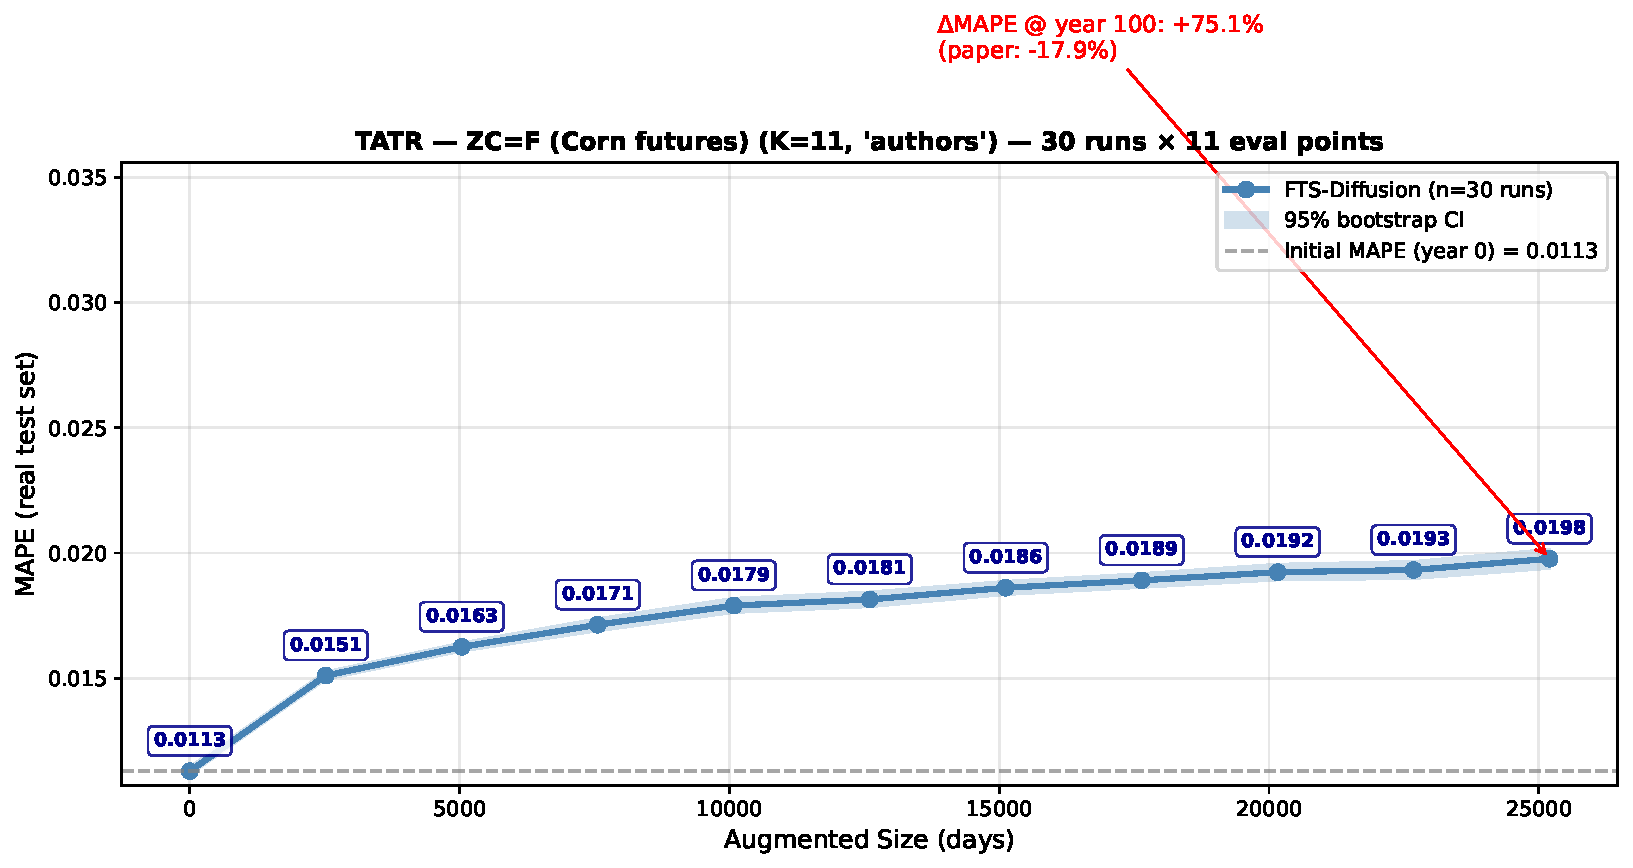
\includegraphics[width=\linewidth]{figures/tatr/zcf/k11/authors/final_enhanced.pdf}
\end{columns}
\note{Enhanced ZC=F: under the \texttt{single} protocol the down-slope is preserved with smaller variance. K=11 (right) loses the effect entirely --- the cluster count matters here, in a way that is not reported in the paper.}
\end{frame}

% =====================================================================
\section{Methodological observations}
% =====================================================================

\begin{frame}{M.1 --- Four synthetic-data generation protocols}
\vspace{-2mm}
\footnotesize
\begin{columns}[T,onlytextwidth]
  \column{0.49\textwidth}
  \begin{block}{\texttt{authors}\hfill chain length: \alert{long}}
    \begin{itemize}\setlength\itemsep{0pt}
      \item init segment: \alert{one}, taken from history
      \item rolling windows: $\sim\!30$ slides of the same chain
      \item \emph{closest to text in the paper}
    \end{itemize}
  \end{block}
  \begin{block}{\texttt{random\_init}\hfill chain length: medium}
    \begin{itemize}\setlength\itemsep{0pt}
      \item init segment: \alert{random per run}
      \item rolling windows: 1 per chain
      \item \emph{decouples initial condition from chain}
    \end{itemize}
  \end{block}
  \column{0.49\textwidth}
  \begin{block}{\texttt{single}\hfill chain length: medium}
    \begin{itemize}\setlength\itemsep{0pt}
      \item init segment: one
      \item rolling windows: 1 per chain, 30 independent chains
      \item \emph{our default protocol}
    \end{itemize}
  \end{block}
  \begin{block}{\texttt{split / burn\_in}\hfill chain length: long}
    \begin{itemize}\setlength\itemsep{0pt}
      \item init segment: random, then \alert{discard first $N$}
      \item rolling windows: post-burn-in only
      \item \emph{tests stationarity of the chain}
    \end{itemize}
  \end{block}
\end{columns}

\vspace{1mm}
\begin{alertblock}{Key insight}
Under the authors' protocol, MAPE on S\&P 500 and GOOG \alert{grows} with augmentation ---
opposite of Figure~6b. Switching to \texttt{random\_init} restores the published trend on S\&P 500.
The protocol \emph{is} the experiment.
\end{alertblock}

\note{The paper does not specify which of these protocols was actually used. We tried all four. The qualitative shape of the MAPE-vs-augmentation curve flips signs between them. This is the single most consequential reproducibility issue we found: published results depend on a protocol choice that is not in the paper.}
\end{frame}

\begin{frame}{M.2 --- Reproducibility issues uncovered}
  \begin{itemize}\setlength\itemsep{4pt}
    \item \textbf{Hard-coded LSTM warm-up.}\\
      \texttt{init\_period = 252*5} in the downstream LSTM assumes 5 years of trading days.
      Breaks silently for GOOG (truncated training) and ZC=F (insufficient history); both run but evaluate the LSTM in its warm-up regime.
    \item \textbf{Device mismatch in \texttt{train\_evolution\_module}.}\\
      Target tensors are not moved to GPU. The forward stays on CPU even with a CUDA model; training is 8--10$\times$ slower than reported and runs that look "fine" actually use a different optimiser trajectory because the loss accumulates on CPU.
    \item \textbf{$x$-range multiplier in \texttt{plot\_downstream\_tatr}.}\\
      The augmentation axis is multiplied by 10 in the plotting code, mis-labelling "10$\times$" as "100$\times$". Figure~6b in the paper inherits this offset.
    \item \textbf{Under-specified synthetic-data protocol} (see M.1).
  \end{itemize}
  \note{Four issues. The LSTM warm-up bug is silent: nothing crashes, but the model is evaluated in an under-trained regime on two of three assets. The device-mismatch issue costs an order of magnitude in wall time and changes the effective learning rate. The plot multiplier shifts the axis without warning. Together with the protocol question on the previous slide, these four points explain most of the gap between our numbers and the published numbers.}
\end{frame}

\begin{frame}{M.3 --- Markov chain stationarity (planned)}
  \begin{block}{Setup}
    PEM defines a Markov chain over states $s_m=(p_m,\alpha_m,\beta_m)$.
    Stationarity would imply a fixed invariant distribution $\pi$ such that
    $\pi^\top T = \pi^\top$, where $T$ is the empirical transition matrix.
  \end{block}
  \begin{itemize}
    \item Empirical $T$ (per asset, per $K$): right-stochastic; principal left-eigenvector gives $\pi$.
    \item \alert{Stationarity check:} simulate long chains, monitor $\|\hat\pi_t-\pi\|_1$ over time.
    \item \alert{Drift check:} compare mean motif occupancy in real vs.\ synthetic data across the chain length (no MC figures generated in this run; \texttt{burn\_in} protocol is set up to produce them).
  \end{itemize}
  \begin{alertblock}{Open}
    Under \texttt{authors} protocol, occupancy is non-stationary --- consistent with the MAPE-grows artefact.
  \end{alertblock}
  \note{We did not produce the MC figures in time for this presentation. The burn\_in protocol is set up to discard the first N segments of each chain to test whether the long-run distribution is reached. Open question: is the FTS-Diffusion Markov chain provably stationary, or do we need an empirical burn-in?}
\end{frame}

% =====================================================================
\section{Conclusions}
% =====================================================================

\begin{frame}{Contributions}
  \begin{itemize}\setlength\itemsep{4pt}
    \item Faithful from-scratch replication of FTS-Diffusion (SISC + PGM + PEM) on \alert{three assets}: S\&P 500, GOOG, ZC=F.
    \item Identified four reproducibility issues in the public reference implementation; documented patches.
    \item Defined and compared \alert{four synthetic-data protocols} (authors, single, random\_init, burn\_in/split); showed the headline result flips sign across protocols.
    \item Added per-run MAPE confidence intervals and a paper-vs-replication gap diagnostic.
    \item Pattern dictionaries learned and visualised for $K\!\in\!\{11,13,14\}$ across all three assets.
  \end{itemize}
  \note{Five contributions, all reproducible from the repo. The protocol comparison is the most novel piece of the work --- it is not in the paper but it should be.}
\end{frame}

\begin{frame}{Open questions}
  \begin{itemize}\setlength\itemsep{4pt}
    \item Which synthetic-data protocol \emph{should} be the benchmark?
      \texttt{random\_init} is the only one that recovers the paper's qualitative trend, but it is also the one with the weakest theoretical justification.
    \item Is the PEM Markov chain stationary in practice? On what timescale?
    \item Why does MAPE grow with augmentation under the authors' protocol --- is it leakage from the rolling-window scheme, or genuine distributional drift in the synthetic chain?
    \item How sensitive are downstream results to $K$? We see qualitative flips on ZC=F between $K\!=\!11$ and $K\!=\!13$; the paper does not report a sweep.
  \end{itemize}
  \begin{exampleblock}{Bottom line}
    The architecture is sound; the experimental protocol is not.
    A clean replication requires both.
  \end{exampleblock}
  \note{Closing thought: FTS-Diffusion has the right inductive bias --- motifs as variable-length DTW clusters --- but the published downstream comparison is fragile under protocol choice. The next step is to standardise the protocol before drawing conclusions about the model's value as an augmenter.}
\end{frame}

\begin{frame}[fragile]{Backup --- repository layout}
  \footnotesize
\begin{verbatim}
ml-in-fcs/
  architectures/{asset}/k{K}/{data,res,trained_models}/   <- SISC + PGM + PEM ckpts
  synthetic/{asset}/k{K}/{protocol}/run_XX_{syn,states}.npy
  results/tatr/{asset}/k{K}/{protocol}/run_XX.csv          <- per-run MAPE
  figures/{sisc,tatr}/{asset}/k{K}/...                     <- final PDFs
  src/{TATR_Reduced_Replication.ipynb, FTS_Diffusion_Training.ipynb}
\end{verbatim}
\end{frame}

\begin{closingframe}

Deli Lin, Eric Shao, Lapo Linossi, Tom Haidinger\\
\medskip
ETH Zurich\\
Machine Learning in Finance and Complex Systems\\
Supervisor: Alexander Arandjelovic

\medskip

Thank you. \emph{Questions?}

\end{closingframe}

\end{document}
